\documentclass{classrep}
\usepackage[utf8]{inputenc}
\usepackage{color}
\usepackage{graphicx}
\usepackage{url}
\usepackage{hyperref}

\studycycle{Informatyka, studia STACJONARNE, I st.}
\coursesemester{VI}

\coursename{Komputerowe systemy rozpoznawania}
\courseyear{2020/2021}

\courseteacher{prof. dr hab. inż. Adam Niewiadomski}
\coursegroup{poniedziałek, 12:00}

\author{
  \studentinfo{Julia Szymańska}{224441} \and
  \studentinfo{Przemysław Zdrzalik}{224466} }

\title{Projekt 2.  Podsumowania lingwistyczne relacyjnych baz danych}

\begin{document}
\maketitle

%%%%%%%%%%%%%%%%%%%%%%%%%%%%%%%%%%%%%%%%
\section{Cel}
Celem projektu jest stworzenie aplikacji pozwalającej na generowanie podsumowań lingwistycznych \cite{przyklad} w oparciu o kwantyfikatory rozmyte \cite{niewiadomskiRozmyte}, co oznacza opisanie danych liczbowych ze zbioru danych \cite{dane} językiem quasi-naturalnym - pozornie naturalnym. \\Przykładem podsumowania lingwistycznego \cite{przyklad} w formie 
\begin{equation} Q\ P\ jest\ S\ [T] \end{equation}
 jest:  \textit{Wiele wypadków jest przy ujemnej temperaturze [0,76]}, gdzie \textit{Q} jest kwantyfikatorem lingwistycznym, \textit{P} podmiotem podsumowań, \textit{S} sumaryzatorem, a \textit{T[0, 1]} stopniem prawdziwości. \\ \newline Przykładem drugiego podsumowania lingwistycznego w formie:
\begin{equation}  Q \ P \ bedacych\ W\ jest\ S\ [T] \end{equation} 
jest: \textit{Wiele wypadków będących podczas deszczu, jest przy ujemnej temperaturze [0.68]}, gdzie \textit{Q} jest kwantyfikatorem lingwistycznym, \textit{P} podmiotem podsumowań, \textit{S} sumaryzatorem, \textit{W} kwantyfikatorem reprezentującym dodatkowe własności obiektów, a \textit{T[0, 1]} stopniem prawdziwości.  \\ \newline
Analizowany zbior danych zawiera liczbowe informacje o ponad 3 milionach wypadków samochodowych w 49 stanach Zjednoczonych Stanów Ameryki, mających miejsce od lutego 2016 do grudnia 2020 \cite{dane}. Zbiór danych składa się z 47 kolumn. W tym celu wykonania podsumowania lingwistycznego zostaną wykorzystane metody logiki rozmytej \cite{fuzzy}. Logika rozmyta pozwala na opisanie wartości zapisanych językiem naturalnym za pomocą zrozumiałych określeń jak: mało, dużo, około połowy. W projekcie zostaną wykorzystane kwantyfikatory lingwistyczne względne takie jak: niewiele, około połowy oraz kwantyfikatory lingwistyczne absolutne takie jak: około jednego, około stu.


%%%%%%%%%%%%%%%%%%%%%%%%%%%%%%%%%%%%%%%%
\section{Charakterystyka podsumowywanej bazy danych}
W programie został użyty zbiór danych \cite{dane} znajdujący się w pliku CSV, który został przekształcony w bazę danych. 

Zbiór danych zawiera informacje o ponad 3 milionach wypadków samochodowych w 49 stanach Zjednoczonych Stanów Ameryki, mających miejsce od lutego 2016 do grudnia 2020. Spośród 47 kolumn znajdujących się w zbiorze danych, wybraliśmy następujące 11 kolumn:
\begin{itemize}
\item Czas rozpoczęcia - Start\_Time - czas rozpoczęcia się wypadku w lokalnej strefie czasowej, przyjmuje wartości od 8 lutego 2016, do 31 grudnia 2020. Wartość kolumny zostanie zamieniona na wartość całkowitą oznaczającą liczbę sekund od początku 1970 roku.
\item Czas zakończenia - End\_Time - czas zakończenia się wypadku w lokalnej strefie czasowej, przyjmuje wartości od 8 lutego 2016, do 1 stycznia 2021. Wartość kolumny zostanie zamieniona na wartość całkowitą oznaczającą liczbę sekund od początku 1970 roku. 
\item Odległość - Distance - długość odcinka ulicy wyrażony w milach, na którego miał wpływ wypadek. Przyjmuje wartości zmiennoprzecinkowe od 0 do 334, gdzie zdecydowana większość danych mieści się w przedziale od 0.00 do 4.00. 
\item Temperatura - Temperature - temperatura powietrza wyrażona w Fahrenheit'ach, w momencie, gdy zdarzył się wypadek.  Przyjmuje wartości zmiennoprzecinkowe od -16.00 do 104.00.  Temperature można opisac jako bardzo zimną, zimną, umiarkowaną, ciepłą, bardzo ciepłą. Oczywiście jest to opis subiektywny.
\item Temperatura odczuwalna - Wind\_Chill - temperatura odczuwalna wyrażona w Fahrenheit'ach, w momencie, gdy zdarzył się wypadek.  Przyjmuje wartości zmiennoprzecinkowe od -16.00 do 101.00. Temperaturę odczuwalną mozna opisać tak samo jak temperaturę.
\item Wilgotność - Humidity - wilgotność powietrza wyrażona w procentach w momencie, gdy zdarzył się wypadek. Przyjmuje wartości zmiennoprzecinkowe od 4.00 do 100.00. 
\item Ciśnienie - Pressure - ciśnienie powietrza wyrażone w inches, w momencie, gdy zdarzył się wypadek. Przyjmuje wartości zmiennoprzecinkowe od 27.00 do 32.00. Ciśnieje można opisac jako wysokie, umiarkowane lub niskie. 
\item Widoczność - Visibiity - widoczność wyrażona w milach, w momencie, gdy zdarzył się wypadek. Przyjmuje wartości zmiennoprzecinkowe od 0.00 do 12.00. 
Widoczność mozna opisać jako dobrą, ograniczoną, słabą.
\item Prędkość wiatru - Wind\_Speed - prędkość wiatru wyrażona w milach na godzinę,  w momencie, gdy zdarzył się wypadek. Przyjmuje wartości zmiennoprzecinkowe od 0.00 do 40.00. Wiatr mozna opisać jako słaby, umiarkowany, silny.
\item Ilość opadów - Principation - ilość opadów wyrażona w inches, w momencie, gdy zdarzył się wypadek. Jeśli opady nie występowały to kolumna przyjmuje wartość nan.  Przyjmuje wartości zmiennoprzecinkowe od 0.00 do 0.50.
\end{itemize}
\ \\
Atrybutom nadawane są opisane zwyczajowe wartości lingwistyczne ze względu na zwiększenie przystępności i ułatwienie szybkiego zrozumienia atrybutu przez człowieka, kiedy ten atrybut nie musi być dokładnie opisany.
Przykładowo temperatura, mimo że zrozumiała dla człowieka w postaci liczbowej, jest łatwiejsza do szybszego zrozumienia w postaci tekstowej, a dla ludzi nie ma dużego znaczenia czy temperatura rózni się o 1 czy 2 stopnie, wystarczy opisać ją słownie tak jak wcześniej podaliśmy jako  bardzo zimną, zimną, umiarkowaną, ciepłą, bardzo ciepłą.

\newpage
\begin{figure}[h!]
 \centering
 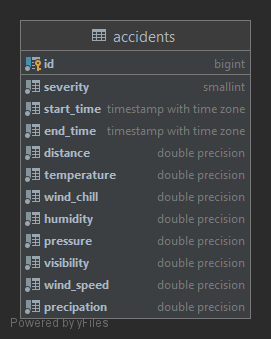
\includegraphics[width=14cm]{accidents.png}
 \vspace{-0.3cm}
 \caption{Tabela reprezentująca omawiane dane wykonana w DBMS Postgresql}
 \label{Wynik klasyfikacji.}
\end{figure}
\newpage


%%%%%%%%%%%%%%%%%%%%%%%%%%%%%%%%%%%%%%%%
\section{Atrybuty i liczności obiektów wyrażone zmiennymi lingwistycznymi}

Poniżej zostaną przedstawione zmiene lingwistyczne \cite{niewiadomskiRozmyte} dla jedenastu atrybutów z bazy danych wraz z przypisanymi etykietami w formie funkcji przynależności oraz wzorów analitycznych. \\

%%%%%%%%%%%%%%%%%%%%%%%%%%%%%%%%%%%%%%%
\subsection{Czas utrudnień w ruchu drogowym spowodowanych przez wypadek}
Na podstawie znajdujących się w bazie danych pól Czas rozpoczęcia (Start\_Time) oraz Czas zakończenia (End\_Time) zostanie obliczony Czas utrudnień w ruchu drogowym (Duration) spowodowanych przez wypadek według wzoru:
\begin{equation}
Duration = End\_Time - Start\_Time
\end{equation}
Przedstawienie Czasu utrudnień w ruchu drogowym (Duration) spowodowanych przez wypadek jako zmiennej lingwistycznej. Do zmiennej lingwistycznej zostały dopasowane etykiety: krótki, średni, długi. 
\begin{equation}
\mu _{czasTrwaniaPonizejGodziny}(x) =  \left\{ \begin{array}{rcl}
\frac{1 - x}{1} & \mbox{dla} & 0 < x \leq 1\\
\end{array}\right.
\end{equation}

\begin{equation}
\mu _{czasTrwaniaOkoloDwochGodzin}(x) =  \left\{ \begin{array}{rcl}
\frac{x}{2} & \mbox{dla} & 0 < x \leq 2\\
\frac{4 - x}{2} & \mbox{dla} & 2 < x \leq 4\\
\end{array}\right.
\end{equation}

\begin{equation}
\mu _{czasTrwaniaOkoloCzterechGodzin}(x) =  \left\{ \begin{array}{rcl}
\frac{x - 2}{2} & \mbox{dla} & 2 < x \leq 4\\
\frac{6 - x}{2} & \mbox{dla} & 4 < x \leq 6\\
\end{array}\right.
\end{equation}

\begin{equation}
\mu _{czasTrwaniaOkoloSzesciuGodzin}(x) =  \left\{ \begin{array}{rcl}
\frac{x - 4}{2} & \mbox{dla} & 4 < x \leq 6\\
\frac{8 - x}{2} & \mbox{dla} & 6 < x \leq 8\\
\end{array}\right.
\end{equation}

\begin{equation}
\mu _{czasTrwaniaPonadSzescGodzin}(x) =  \left\{ \begin{array}{rcl}
\frac{x - 6}{2} & \mbox{dla} & 6 < x \leq 8\\
 1 & \mbox{dla} & 8 \leq  x \\
\end{array}\right.
\end{equation}

gdzie: \(\mu _{czasTrwaniaPonizejGodziny}\), \(\mu _{czasTrwaniaOkoloDwochGodzin}\), \(\mu _{czasTrwaniaOkoloCzterechGodzin}\), \(\mu _{czasTrwaniaOkoloSzesciuGodzin}\), \(\mu _{czasTrwaniaPonadSzescGodzin}\) - funkcje przynależności, \textit{x} - czas trwania wypadku. 
\begin{figure}[h!]
 \centering
 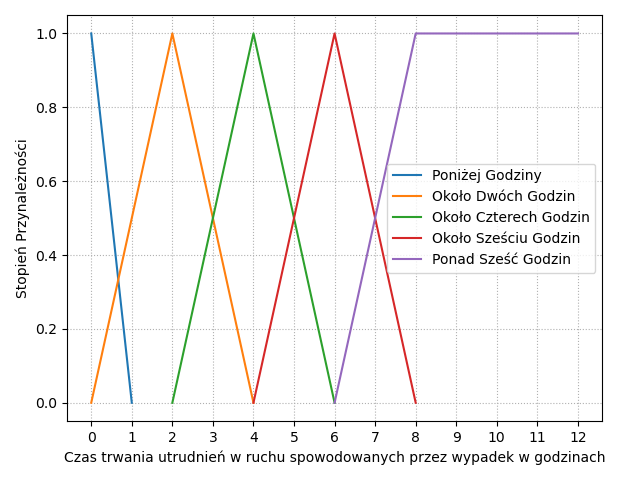
\includegraphics[width=14cm]{FunkcjaPrzynaleznosciCzasTrwania.png}
 \vspace{-0.3cm}
 \caption{Wykres funkcji przynależności zbiorów rozmytych ilustrujących wartości zmiennej lingwistycznej czas utrudnień w ruchu drogowym (Duration) spowodowanych przez wypadek. }
 \label{rysunek do eksperymentu 1 wariantu 1}
\end{figure}
\newpage


%%%%%%%%%%%%%%%%%%%%%%%%%%%%%%%%%%%%%%%%
\subsection{Odległość}

Przedstawienie odległości jako zmiennej lingwistycznej. Do zmiennej lingwistycznej zostały dopasowane etykiety: krótki, długi. 
\begin{equation}
\mu _{OdlegloscPonizejPolMili}(x) =  \left\{ \begin{array}{rcl}
 1 & \mbox{dla} & x  \leq 0.5 \\
\end{array}\right.
\end{equation}

\begin{equation}
\mu _{OdlegloscOkoloJednejMili}(x) =  \left\{ \begin{array}{rcl}
x & \mbox{dla} & 0 < x \leq 1\\
2 - x & \mbox{dla} & 1 < x \leq 2\\
\end{array}\right.
\end{equation}

\begin{equation}
\mu _{OdlegloscOkoloTrzechMili}(x) =  \left\{ \begin{array}{rcl}
\frac{x - 1}{2} & \mbox{dla} & 1 < x \leq 3\\
\frac{5 - x}{2} & \mbox{dla} & 3 < x \leq 5\\
\end{array}\right.
\end{equation}

\begin{equation}
\mu _{OdlegloscPonadTrzyMile}(x) =  \left\{ \begin{array}{rcl}
\frac{x - 3}{2} & \mbox{dla} & 3 < x \leq 5\\
1 & \mbox{dla} & 5 \leq x \\
\end{array}\right.
\end{equation}

gdzie: \(\mu _{OdlegloscPonizejPolMili}\), \(\mu _{OdlegloscOkoloJednejMili}\), \(\mu _{OdlegloscOkoloTrzechMili}\), \(\mu _{OdlegloscPonadTrzyMile}\) - funkcje przynależności, \textit{x} - odleglość. 

\begin{figure}[h!]
 \centering
 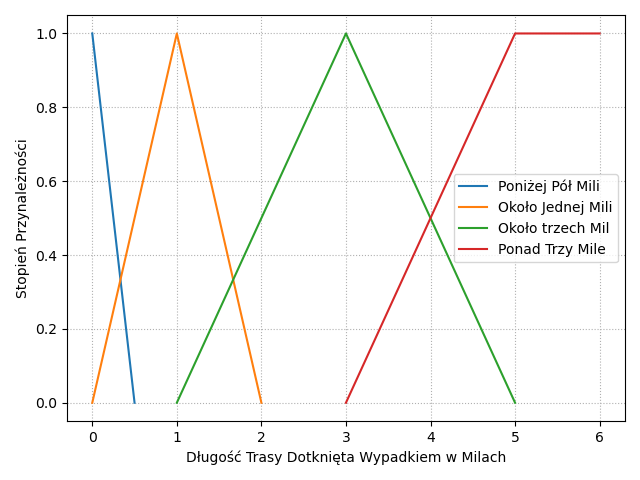
\includegraphics[width=14cm]{FunkcjaPrzynaleznosciOdleglosc.png}
 \vspace{-0.3cm}
 \caption{Wykres funkcji przynależności zbiorów rozmytych ilustrujących wartości zmiennej lingwistycznej odległości. }
 \label{rysunek do eksperymentu 1 wariantu 1}
\end{figure}
\newpage

%%%%%%%%%%%%%%%%%%%%%%%%%%%%%%%%%%%%%%%%
\subsection{Tempertura i temperatura odczuwalna}
Przedstawienie temperatury oraz temperatury odczuwalnej jako zmiennej lingwistycznej. Do zmiennej lingwistycznej zostały dopasowane etykiety: bardzo zimno, zimno, umiarkowanie, ciepło, bardzo ciepło. 
\begin{equation}
\mu _{temperaturaBardzoZimno}(x) =  \left\{ \begin{array}{rcl}
 1 & \mbox{dla} & x  \leq 14 \\
\frac{23 - x}{9} & \mbox{dla} & 14 < x \leq 23\\
\end{array}\right.
\end{equation}

\begin{equation}
\mu _{temperaturaZimno}(x) =  \left\{ \begin{array}{rcl}
\frac{x - 14}{9} & \mbox{dla} & 14 < x \leq 23\\
1 & \mbox{dla} & 23 < x < 44\\
\frac{54 - x}{10} & \mbox{dla} & 44 < x \leq 54\\
\end{array}\right.
\end{equation}

\begin{equation}
\mu _{temperaturaUmiarkowanie}(x) =  \left\{ \begin{array}{rcl}
\frac{x - 44}{10} & \mbox{dla} & 44 < x \leq 54\\
1 & \mbox{dla} & 54 < x < 63\\
\frac{71 - x}{8} & \mbox{dla} & 63 < x \leq 71\\
\end{array}\right.
\end{equation}

\begin{equation}
\mu _{temperaturaCieplo}(x) =  \left\{ \begin{array}{rcl}
\frac{x - 63}{8} & \mbox{dla} & 63 < x \leq 71\\
1 & \mbox{dla} & 71 < x < 80\\
\frac{90 - x}{10} & \mbox{dla} & 80 < x \leq 90\\
\end{array}\right.
\end{equation}

\begin{equation}
\mu _{temperaturaBardzoCieplo}(x) =  \left\{ \begin{array}{rcl}
\frac{x - 80}{10} & \mbox{dla} & 80 < x \leq 90\\
1 & \mbox{dla} & 90 \leq x\\
\end{array}\right.
\end{equation}

gdzie: \(\mu _{temperaturaBardzoZimna}\), \(\mu _{temperaturaZimna}\), \(\mu _{temperaturaUmiarkowana}\), \(\mu _{temperaturaCiepla}\), \(\mu _{temperaturaBardzoCiepla}\) - funkcje przynależności, \textit{x} - temperatura, temperatura odczuwalna. 


\begin{figure}[h!]
 \centering
 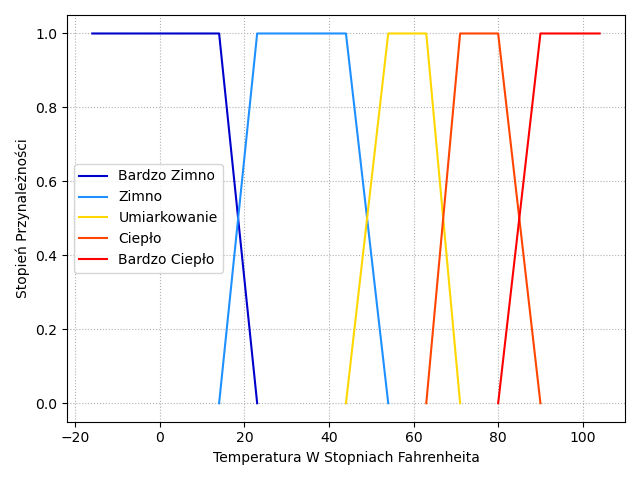
\includegraphics[width=14cm]{FunkcjaPrzynaleznosciTemperatura.png}
 \vspace{-0.3cm}
 \caption{Wykres funkcji przynależności zbiorów rozmytych ilustrujących wartości zmiennej lingwistycznej temperatury. }
 \label{rysunek do eksperymentu 1 wariantu 1}
\end{figure}
\newpage



%%%%%%%%%%%%%%%%%%%%%%%%%%%%%%%%%%%%%%%%
\subsection{Wilgotność}
Przedstawienie wilgotności jako zmiennej lingwistycznej. Do zmiennej lingwistycznej zostały dopasowane etykiety: suche, umiarkowane, wilgotne. 

\begin{equation}
\mu _{wilgotnoscBardzoSuche}(x) =   exp( \frac{- (x - 4)^2}{128} )
\end{equation}

\begin{equation}
\mu _{wilgotnoscSuche}(x) =   exp( \frac{- (x - 25)^2}{128} )
\end{equation}

\begin{equation}
\mu _{wilgotnoscUmiarkowane}(x) =   exp( \frac{- (x - 50)^2}{128} )
\end{equation}

\begin{equation}
\mu _{wilgotnoscWilgotne}(x) =   exp( \frac{- (x - 75)^2}{128} )
\end{equation}

\begin{equation}
\mu _{wilgotnoscBardzoWilgotne}(x) =  \left\{ \begin{array}{rcl}
\frac{x - 60}{10} & \mbox{dla} & 60 < x \leq 70\\
1 & \mbox{dla} & 70 < x < 80\\
\frac{90 - x}{10} & \mbox{dla} & 80 < x \leq 90\\
\end{array}\right.
\end{equation}

gdzie: \(\mu _{wilgotnoscBardzoSuche}\), \(\mu _{wilgotnoscSuche}\), \(\mu _{wilgotnoscUmiarkowane}\), \(\mu _{wilgotnoscWilgotne}\), \(\mu _{wilgotnoscBardzoWilgotne}\) - funkcje przynależności, \textit{x} - wilgotność. 

\begin{figure}[h!]
 \centering
 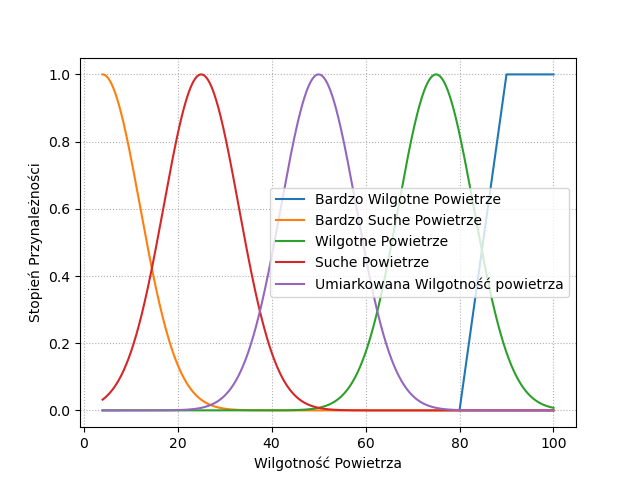
\includegraphics[width=14cm]{FunkcjaPrzynaleznosciWilgotnosc.png}
 \vspace{-0.3cm}
 \caption{Wykres funkcji przynależności zbiorów rozmytych ilustrujących wartości zmiennej lingwistycznej wilgotności. }
 \label{rysunek do eksperymentu 1 wariantu 1}
\end{figure}
\newpage


%%%%%%%%%%%%%%%%%%%%%%%%%%%%%%%%%%%%%%%%
\subsection{Ciśnienie}
Przedstawienie ciśnienia jako zmiennej lingwistycznej. Do zmiennej lingwistycznej zostały dopasowane etykiety: niskie, umiarkowane, wysokie. 

\begin{equation}
\mu _{cisnienieBardzoNiskie}(x) =   exp( \frac{- (x - 27)^2}{0.18} )
\end{equation}

\begin{equation}
\mu _{cisnienieNiskie}(x) =   exp( \frac{- (x - 27.75)^2}{0.18} )
\end{equation}

\begin{equation}
\mu _{cisnienieUmiarkowane}(x) =   exp( \frac{- (x - 28.75)^2}{0.18} )
\end{equation}

\begin{equation}
\mu _{cisnienieWysokie}(x) =   exp( \frac{- (x - 29.75)^2}{0.18} )
\end{equation}

\begin{equation}
\mu _{cisnienieBardzoWysokie}(x) =  \left\{ \begin{array}{rcl}
\frac{x - 30}{0.5} & \mbox{dla} & 30 < x \leq 30.5\\
1 & \mbox{dla} & 30.5 \leq x\\
\end{array}\right.
\end{equation}


gdzie: \(\mu _{cisnienieBardzoNiskie}\), \(\mu _{cisnienieNiskie}\), \(\mu _{cisnienieUmiarkowane}\), \(\mu _{cisnienieWysokie}\), \(\mu _{cisnienieBardzoWysokie}\) - funkcje przynależności, \textit{x} - ciśnienie. 

\begin{figure}[h!]
 \centering
 \includegraphics[width=14cm]{FunkcjaPrzynaleznosciCiśnienie.png}
 \vspace{-0.3cm}
 \caption{Wykres funkcji przynależności zbiorów rozmytych ilustrujących wartości zmiennej lingwistycznej ciśneinia. }
 \label{rysunek do eksperymentu 1 wariantu 1}
\end{figure}
\newpage



%%%%%%%%%%%%%%%%%%%%%%%%%%%%%%%%%%%%%%%%
\subsection{Widoczność}
Przedstawienie widoczności jako zmiennej lingwistycznej. Do zmiennej lingwistycznej zostały dopasowane etykiety: brak, słaba, ograniczona, dobra. 
\begin{equation}
\mu _{widocznoscBrak}(x) =   1 \ \ dla \ \ x  = 0
\end{equation}

\begin{equation}
\mu _{widocznoscSlaba}(x) =  \left\{ \begin{array}{rcl}
 1 & \mbox{dla} & x  \leq 0.1 \\
\frac{0.1 - x}{0.2} & \mbox{dla} & 0.1 < x \leq 0.3\\
\end{array}\right.
\end{equation}

\begin{equation}
\mu _{widocznoscOgraniczona}(x) =  \left\{ \begin{array}{rcl}
\frac{x - 0.1}{0.2} & \mbox{dla} & 0.1 < x \leq 0.3\\
1 & \mbox{dla} & 0.3 < x < 0.7\\
\frac{1 - x}{0.3} & \mbox{dla} & 0.7 < x \leq1\\
\end{array}\right.
\end{equation}

\begin{equation}
\mu _{widocznoscDobra}(x) =  \left\{ \begin{array}{rcl}
\frac{x - 0.7}{0.3} & \mbox{dla} & 0.7 < x \leq 1\\
1 & \mbox{dla} & 1 < x < 2\\
\frac{3 - x}{1} & \mbox{dla} & 2 < x \leq 3\\
\end{array}\right.
\end{equation}

\begin{equation}
\mu _{widocznoscPelna}(x) =  \left\{ \begin{array}{rcl}
\frac{x - 3}{1} & \mbox{dla} & 2 < x \leq 3\\
1 & \mbox{dla} & 3 \leq x\\
\end{array}\right.
\end{equation}

gdzie: \(\mu _{widocznoscBrak}\), \(\mu _{widocznoscSlaba}\), \(\mu _{widocznoscOgraniczona}\), \(\mu _{widocznoscDobra}\), \(\mu _{widocznoscPelna}\)  - funkcje przynależności, \textit{x} - widoczność. 

\begin{figure}[h!]
 \centering
 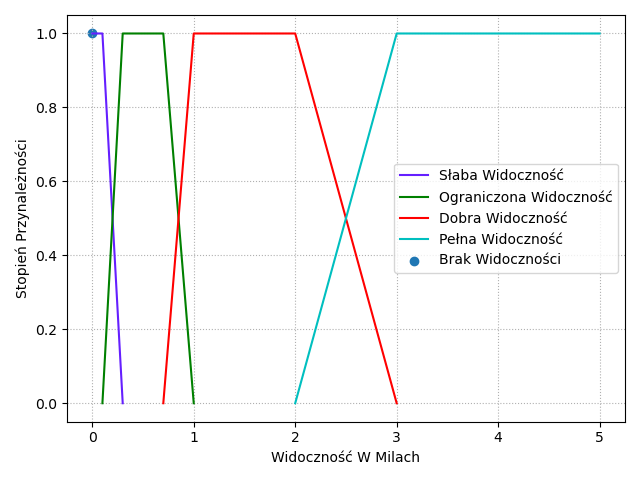
\includegraphics[width=14cm]{FunkcjaPrzynaleznosciWidocznosc.png}
 \vspace{-0.3cm}
 \caption{Wykres funkcji przynależności zbiorów rozmytych ilustrujących wartości zmiennej lingwistycznej widoczności. }
 \label{rysunek do eksperymentu 1 wariantu 1}
\end{figure}
\newpage


%%%%%%%%%%%%%%%%%%%%%%%%%%%%%%%%%%%%%%%%
\subsection{Prędkość wiatru}
Przedstawienie predkości wiatru jako zmiennej lingwistycznej. Do zmiennej lingwistycznej zostały dopasowane etykiety: brak, słaby, umiarkowany, silny, wicher, huragan. 

\begin{equation}
\mu _{wiatrBrak}(x) =   1 \ \ dla \ \ x  = 0
\end{equation}

\begin{equation}
\mu _{wiatrSlaby}(x) =  \left\{ \begin{array}{rcl}
 1 & \mbox{dla} & x  \leq 3 \\
\frac{3- x}{0.5} & \mbox{dla} & 3 < x \leq 3.5\\
\end{array}\right.
\end{equation}

\begin{equation}
\mu _{wiatrUmiarkowany}(x) =  \left\{ \begin{array}{rcl}
\frac{x - 3}{0.5} & \mbox{dla} & 3 < x \leq 3.5\\
1 & \mbox{dla} & 3.5 < x < 8\\
\frac{9 - x}{1} & \mbox{dla} & 8 < x \leq 9\\
\end{array}\right.
\end{equation}

\begin{equation}
\mu _{wiatrSilny}(x) =  \left\{ \begin{array}{rcl}
\frac{x - 8}{1} & \mbox{dla} & 8 < x \leq 9\\
1 & \mbox{dla} & 9 < x < 17\\
\frac{20 - x}{3} & \mbox{dla} & 17 < x \leq 20\\
\end{array}\right.
\end{equation}

\begin{equation}
\mu _{wiatrWicher}(x) =  \left\{ \begin{array}{rcl}
\frac{x - 17}{3} & \mbox{dla} & 17 < x \leq 20\\
1 & \mbox{dla} & 20 < x < 27\\
\frac{30 - x}{3} & \mbox{dla} & 27 < x \leq 30\\
\end{array}\right.
\end{equation}

\begin{equation}
\mu _{wiatrHuragan}(x) =  \left\{ \begin{array}{rcl}
\frac{x - 40}{10} & \mbox{dla} & 30 < x \leq 40\\
1 & \mbox{dla} & 40 \leq x\\
\end{array}\right.
\end{equation}

gdzie: \(\mu _{wiatrBrak}\), \(\mu _{wiatrSlaby}\), \(\mu _{wiatrUmiarkowany}\), \(\mu _{wiatrSilny}\), \(\mu _{wiatrWicher}\), \(\mu _{wiatrHuragan}\)  - funkcje przynależności, \textit{x} - prędkość wiatru. 

\begin{figure}[h!]
 \centering
 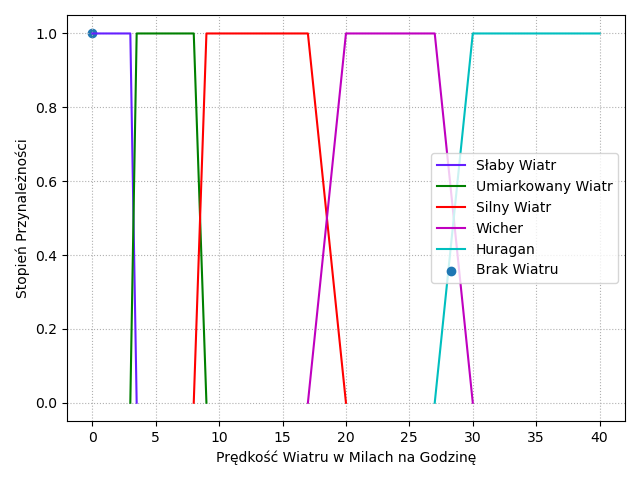
\includegraphics[width=14cm]{FunkcjaPrzynaleznosciPredkoscWiatru.png}
 \vspace{-0.3cm}
 \caption{Wykres funkcji przynależności zbiorów rozmytych ilustrujących wartości zmiennej lingwistycznej prędkości wiatru. }
 \label{rysunek do eksperymentu 1 wariantu 1}
\end{figure}
\newpage



%%%%%%%%%%%%%%%%%%%%%%%%%%%%%%%%%%%%%%%%
\subsection{Opady}
Przedstawienie opadów jako zmiennej lingwistycznej. Do zmiennej lingwistycznej zostały dopasowane etykiety: brak, niewielkie, umiarkowane, duże. 

\begin{equation}
\mu _{opadyBrak}(x) =   1 \ \ dla \ \ x  = 0
\end{equation}

\begin{equation}
\mu _{opadyNiewielkie}(x) =  \left\{ \begin{array}{rcl}
 1 & \mbox{dla} & x  \leq 0.1 \\
\frac{0.1- x}{0.1} & \mbox{dla} & 0.1 < x \leq 0.2\\
\end{array}\right.
\end{equation}

\begin{equation}
\mu _{opadyUmiarkowane}(x) =  \left\{ \begin{array}{rcl}
\frac{x - 0.1}{0.1} & \mbox{dla} & 0.1 < x \leq 0.2\\
1 & \mbox{dla} & 0.2 < x < 0.3\\
\frac{0.35 - x}{0.05} & \mbox{dla} & 0.3 < x \leq 0.35\\
\end{array}\right.
\end{equation}


\begin{equation}
\mu _{opadyDuze}(x) =  \left\{ \begin{array}{rcl}
\frac{x - 0.35}{0.05} & \mbox{dla} & 0.3 < x \leq 0.35\\
1 & \mbox{dla} & 0.35 < x < 0.4\\
\frac{0.45 - x}{0.05} & \mbox{dla} & 0.4 < x \leq 0.45\\
\end{array}\right.
\end{equation}

\begin{equation}
\mu _{opadyBardzoDuze}(x) =  \left\{ \begin{array}{rcl}
\frac{x - 0.4}{0.05} & \mbox{dla} & 0.4 < x \leq 0.45\\
1 & \mbox{dla} & 0.45 \leq x\\
\end{array}\right.
\end{equation}

gdzie: \(\mu _{opadyBrak}\), \(\mu _{opadyNiewielkie}\), \(\mu _{opadyUmiarkowane}\), \(\mu _{opadyDuze}\), \(\mu _{opadyBardzoDuze}\)  - funkcje przynależności, \textit{x} - opady. 

\begin{figure}[h!]
 \centering
 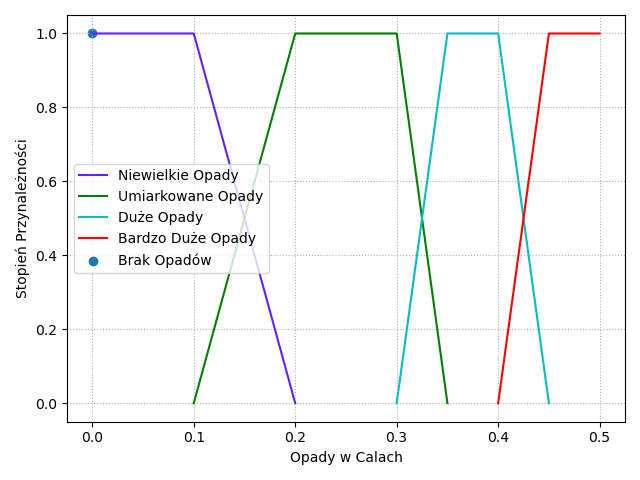
\includegraphics[width=14cm]{FunkcjaPrzynaleznosciOpady.png}
 \vspace{-0.3cm}
 \caption{Wykres funkcji przynależności zbiorów rozmytych ilustrujących wartości zmiennej lingwistycznej opadów. }
 \label{rysunek do eksperymentu 1 wariantu 1}
\end{figure}
\newpage


%%%%%%%%%%%%%%%%%%%%%%%%%%%%%%%%%%%%%%%%
\subsection{Kwantyfikator lingwistyczny względny}
Do kwantyfikatora lingwistycznego względnego \cite{niewiadomskiRozmyte} zostały dopasowane etykiety: niewiele, około 1/4, około połowy, większość, prawie wszystkie. 

\begin{equation}
\mu _{niewiele}(x) =   exp( \frac{- x^2}{0.02} )
\end{equation}

\begin{equation}
\mu _{okoloJednejCzwartej}(x) =   exp( \frac{- (x - 0.25)^2}{0.02} )
\end{equation}

\begin{equation}
\mu _{okoloPolowy}(x) =   exp( \frac{- (x - 0.5)^2}{0.02} )
\end{equation}

\begin{equation}
\mu _{wiekszosc}(x) =   exp( \frac{- (x - 0.75)^2}{0.02} )
\end{equation}

\begin{equation}
\mu _{prawieWszystkie}(x) =   exp( \frac{- (x - 1)^2}{0.02} )
\end{equation}

gdzie: \(\mu _{niewiele}\), \(\mu _{okoloJednejCzwartej}\), \(\mu _{okoloPolowy}\), \(\mu _{wiekszosc}\), \(\mu _{prawieWszystkie}\)  - kwantyfikatory, \textit{x} - stosunek liczby obiektów posiadających cechę do wszystkich rozważanych obiektów. 

\begin{figure}[h!]
 \centering
 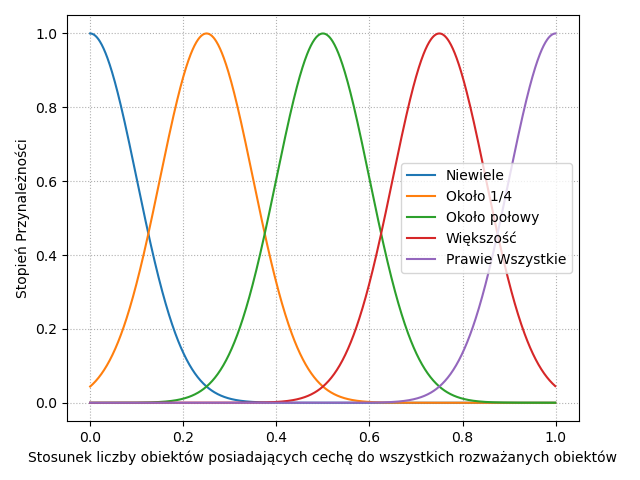
\includegraphics[width=14cm]{kwantyfikatory.png}
 \vspace{-0.3cm}
 \caption{Wykres funkcji przynależności kwantyfikatorów lingwistycznych względnych. }
 \label{rysunek do eksperymentu 1 wariantu 1}
\end{figure}
\newpage

%%%%%%%%%%%%%%%%%%%%%%%%%%%%%%%%%%%%%%%%
\subsection{Kwantyfikator lingwistyczny absolutny}
Do kwantyfikatora lingwistycznego absolutnego \cite{niewiadomskiRozmyte} zostały dopasowane etykiety: poniżej 10, około 50, około 100, między 100 a 200, około 200, ponad 200. 

\begin{equation}
\mu _{ponizej10}(x) =  \left\{ \begin{array}{rcl}
\frac{10 - x}{10} & \mbox{dla} & 0 < x \leq 10\\
\end{array}\right.
\end{equation}

\begin{equation}
\mu _{okolo20}(x) =  \left\{ \begin{array}{rcl}
\frac{x}{20} & \mbox{dla} & 0 < x \leq 20\\
\frac{40 - x}{20} & \mbox{dla} & 0 < x \leq 40\\
\end{array}\right.
\end{equation}

\begin{equation}
\mu _{okolo50}(x) =  \left\{ \begin{array}{rcl}
\frac{x - 10}{30} & \mbox{dla} & 10 < x \leq40\\
1 & \mbox{dla} & 40 < x < 60\\
\frac{90 - x}{30} & \mbox{dla} & 60 < x \leq 90\\
\end{array}\right.
\end{equation}

\begin{equation}
\mu _{okolo100}(x) =  \left\{ \begin{array}{rcl}
\frac{x - 50}{40} & \mbox{dla} & 50 < x \leq 90\\
1 & \mbox{dla} & 90 < x < 110\\
\frac{150 - x}{50} & \mbox{dla} & 110 < x \leq 150\\
\end{array}\right.
\end{equation}

\begin{equation}
\mu _{miedzy100A200}(x) =  \left\{ \begin{array}{rcl}
\frac{x}{50} & \mbox{dla} & 100 < x \leq 150\\
\frac{200- x}{50} & \mbox{dla} & 150 < x \leq 200\\
\end{array}\right.
\end{equation}

\begin{equation}
\mu _{okolo200}(x) =  \left\{ \begin{array}{rcl}
\frac{x - 150}{40} & \mbox{dla} & 150 < x \leq 190\\
1 & \mbox{dla} & 190 < x < 210\\
\frac{250 - x}{40} & \mbox{dla} & 210 < x \leq 250\\
\end{array}\right.
\end{equation}

\begin{equation}
\mu _{Ponad200}(x) =  \left\{ \begin{array}{rcl}
\frac{x - 200}{50} & \mbox{dla} & 200 < x \leq 250\\
1 & \mbox{dla} & 250 < x < 300\\
\frac{300 - x}{50} & \mbox{dla} & 300 < x \leq 350\\
\end{array}\right.
\end{equation}

\begin{equation}
\mu _{Okolo500}(x) =  \left\{ \begin{array}{rcl}
\frac{x - 300}{200} & \mbox{dla} & 300 < x \leq 400\\
1 & \mbox{dla} & 400 < x < 600\\
\frac{600 - x}{100} & \mbox{dla} & 600 < x \leq 700\\
\end{array}\right.
\end{equation}

\begin{equation}
\mu _{Okolo1000}(x) =  \left\{ \begin{array}{rcl}
\frac{x - 600}{200} & \mbox{dla} & 600 < x \leq 800\\
1 & \mbox{dla} & 800 < x < 1200\\
\frac{1200 - x}{200} & \mbox{dla} & 1200 < x \leq 1400\\
\end{array}\right.
\end{equation}

\begin{equation}
\mu _{Okolo2000}(x) =  \left\{ \begin{array}{rcl}
\frac{x - 1200}{400} & \mbox{dla} & 1200 < x \leq 1600\\
1 & \mbox{dla} & 1600 < x < 2400\\
\frac{2400 - x}{400} & \mbox{dla} & 2400 < x \leq 2800\\
\end{array}\right.
\end{equation}

\begin{equation}
\mu _{Okolo3500}(x) =  \left\{ \begin{array}{rcl}
\frac{x - 2400}{400} & \mbox{dla} & 2400 < x \leq 2800\\
1 & \mbox{dla} & 2800 < x < 4200\\
\frac{4200 - x}{400} & \mbox{dla} & 4200 < x \leq 4600\\
\end{array}\right.
\end{equation}

gdzie: \(\mu _{ponizej10}\), \(\mu _{okolo20}\), \(\mu _{okolo50}\), \(\mu _{okolo100}\), \(\mu _{miedzy100A200}\), \(\mu _{okolo200}\), \(\mu _{Ponad200}\),  \(\mu _{Okolo500}\), \(\mu _{Okolo1000}\),  \(\mu _{Okolo200}\), \(\mu _{Okolo3500}\),  - kwantyfikatory absolutne, \textit{x} - absolutna wartość liczby obiektów posiadających cechę. 

\begin{figure}[h!]
 \centering
 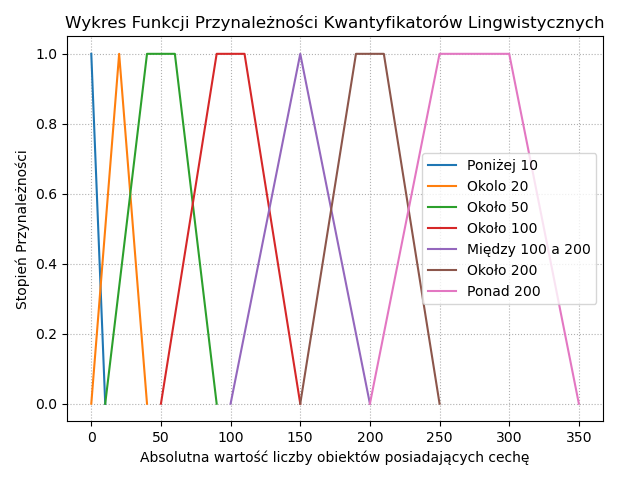
\includegraphics[width=14cm]{kwantyfikatory_absolutny_2.png}
 \vspace{-0.3cm}
 \caption{Wykres funkcji przynależności kwantyfikatorów lingwistycznych absolutnych od wartości 0 do 350. }
 \label{kwantyfikatory_lingwistyczne_absolutne}
\end{figure}


\begin{figure}[h!]
 \centering
 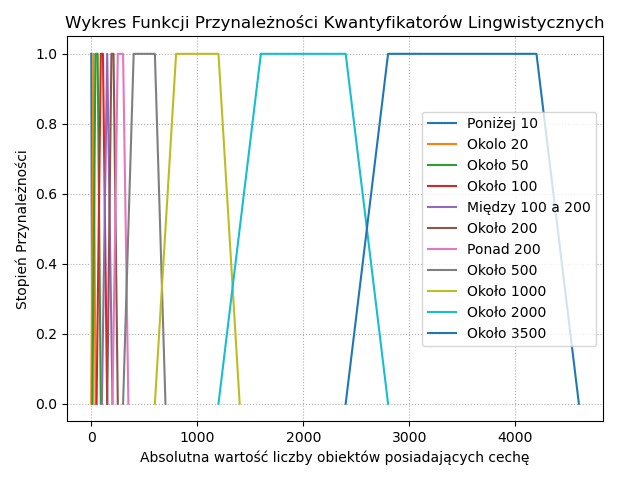
\includegraphics[width=14cm]{kwantyfikatory_absolutny.png}
 \vspace{-0.3cm}
 \caption{Wykres funkcji przynależności kwantyfikatorów lingwistycznych absolutnych. }
 \label{kwantyfikatory_lingwistyczne_absolutne}
\end{figure}
\newpage

%%%%%%%%%%%%%%%%%%%%%%%%%%%%%%%%%%%%%%%%
\section{Narzędzia obliczeniowe: projekt (wybór, implementacja) i diagram UML pakietu obliczeń rozmytych. Diagram UML generatora podsumowań}
\subsection{Diagram pakietu obliczeń rozmytych}

\begin{figure}[h!]
 \centering
 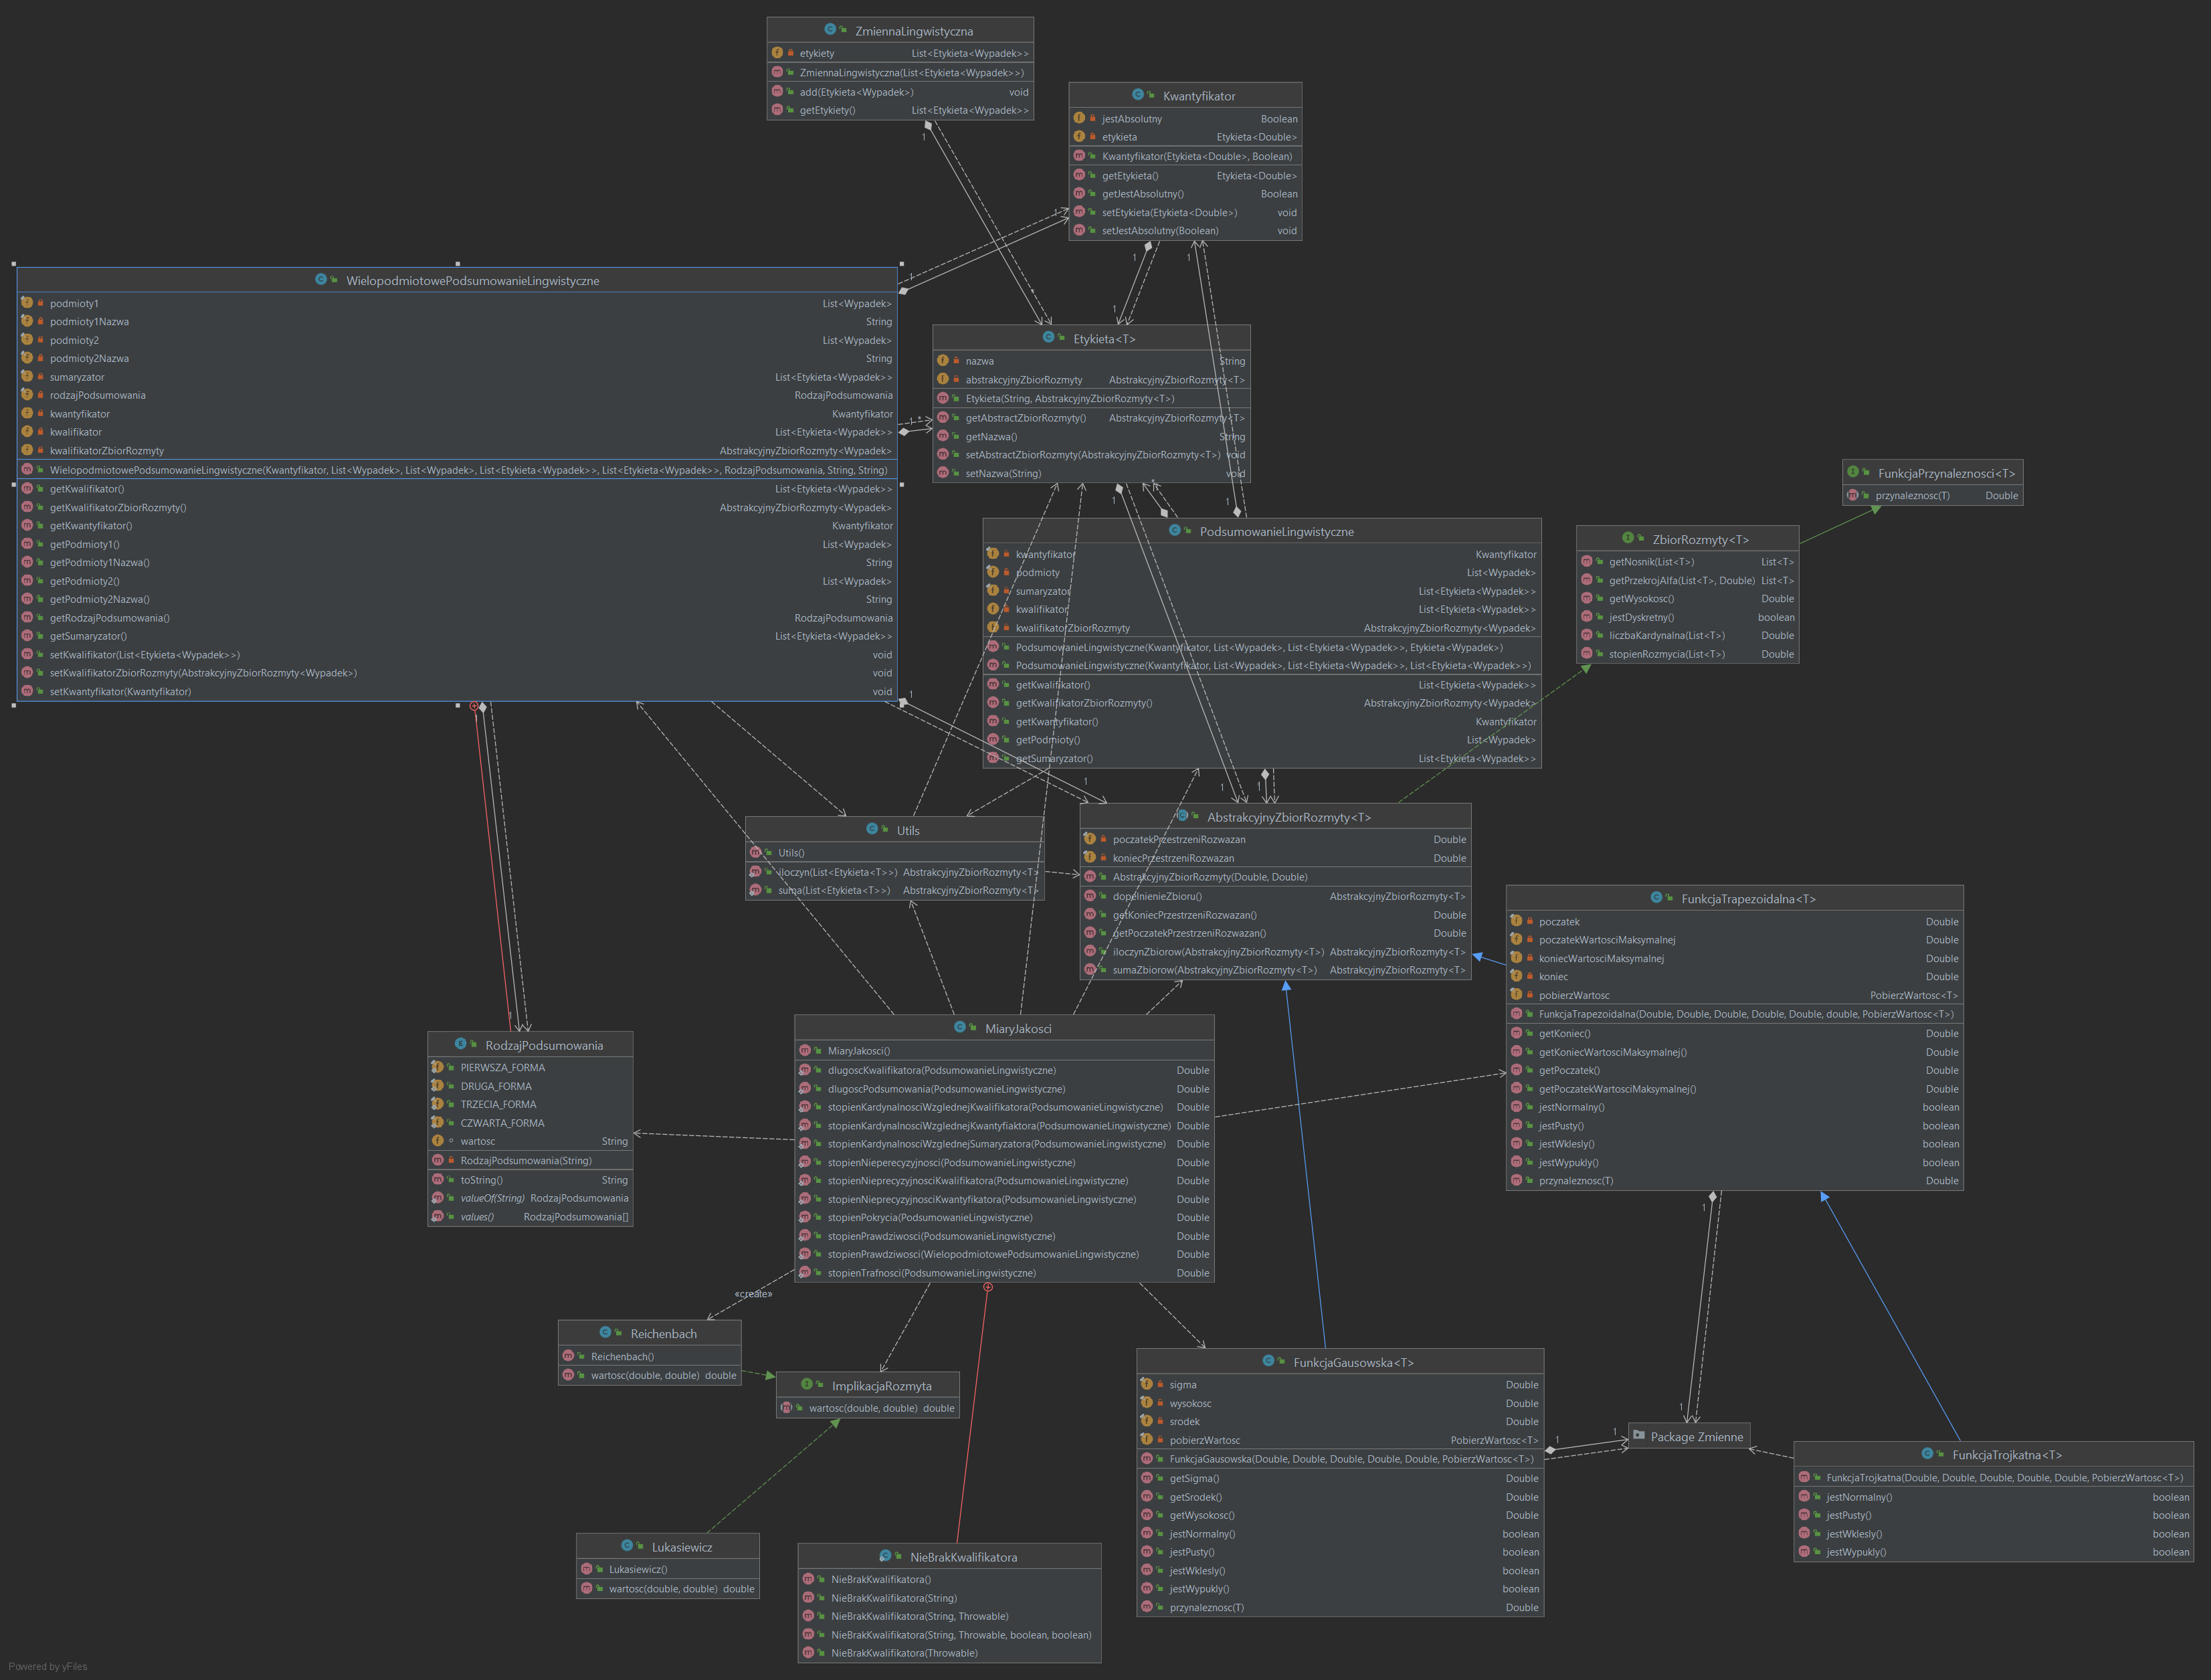
\includegraphics[width=14cm]{uml.png}
 \vspace{-0.3cm}
 \caption{Diagram uml pakietu obliczeń rozmytych. }
 \label{uml_obliczenia}
\end{figure}
\newpage

Program został wykonany w języku Java 11 LTS z użyciem narzędzia Maven. W celu wykonania projektu stworzyliśmy własny pakiet obliczeń rozmytych - obliczeniaRozmyte. Pakiet ten jest przystosowany do pracy przy użyciu naszego dyskretnego zbioru danych o wypadkach samochodowych w Stanach Zjednoczonych Ameryki. Pakiet posiada klasy oraz interfejsy niezbędne do wykonywania obliczeń rozmytych i generowania podsumowań lingwistycznych. Interfejs FunkcjaPrzynaleznosci posiada jedną metodę pozwalającą na obliczenie przynależności obiektu do zbioru \cite{broniarska}.
Interfejs ten rozszerzany jest przez interfejs ZbiorRozmyty który pozwala na obliczenie różnych własności zbioru rozmytego: wysokość \cite{fuzzy}, liczbę kardynalna \cite{fuzzy}, stopień rozmycia \cite{niewiadomski19} oraz pozwala na pobranie zbiorów nierozmytych będących odpowiednio nośnikiem \cite{broniarska} i przekrojem alfa zbioru rozmytego \cite{broniarska}. Interfejs ten jest implementowany przez abstrakcyjną klasę AbstrakcyjnyZbiorRozmyty posiadającą informacje o początku i końcu przestrzeni rozważań \cite{fuzzy}, i pozwalającą na wyznaczenie dopełnienia zbioru oraz iloczynu i sumy zbioru z innym zbiorem rozmytym \cite{fuzzy}. Klasa ta implementowana jest przez klasy odpowiadające odpowiednio FunkcjaGaussowskiej \cite{broniarska} i FunkcjaTrapezoidalna \cite{broniarska}, a po FunkcjaTrapezoidalna nastepnie dziedziczy FunkcjaTrojkatna \cite{broniarska}. W celu pobrania odpowiedniego pola z obiektu w celu obliczenia przynależności klasy implementujące AbstrakcyjnyZbiorRozmyty posiadają jako swoje pole interfejs PobierzWartosc, który wybiera z klasy odpowiednie pole podlegające podsumowaniu. Odpowiednie implementacje klasy AbstrakcyjnyZbiorRozmyty posiadają też informacje o tym czy zbiór przez nie reprezentowany jest normalny \cite{broniarska}, pusty \cite{broniarska}, wklęsły \cite{broniarska} lub wypukły \cite{broniarska}.
ZbiorRozmyty jest natępnie używany przy tworzeniu Etykiety \cite{niewiadomski19}, gdzie każda posiada swoją nazwę i odpowedni zbiór rozmyty. Używając Etykiet reprezentujemy Kwantyfikatory \cite{niewiadomski19}, kwalifikatory \cite{niewiadomski19} oraz sumaryzatory \cite{niewiadomski19}. Do obliczania iloczynu lub sumy wielu zbiorów rozmytych używamy klasy Utils posiadającą odpowiednie statyczne metody. Kwantyfikator posiada etykietę oraz informacje czy jest on absolutny \cite{niewiadomski19}. Klasa ZmiennaLingwistyczna reprezentuje zmienną lingwistyczną poprzez listę Etykiet. Klasa PodsumowanieLingwistyczne reprezentuje podsumowanie lingiwstyczne poprzez kwantyfikator, kwalifikator, sumaryzator oraz podmioty. Dla każdego podsumowania jednopodmiotowego możemy policzyć miary \textit{T\textsubscript{1}} - \textit{T\textsubscript{11}} korzystając z klasy MiaryJakosci, natomiast dla podsumowania wielopodmiotowego możemy policzyć \textit{T\textsubscript{1}}. Pakiet zawiera enum RodzajPodsumowania zawierający cztery nazwy rodzajów podsumowania, klasa WielopodmiotowePodsumowanieLingwistyczne korzysta z enum w celu wygenerowania odpowiedniego podsumowania wielopodmiotowego. Klasa WielopodmiotowePodsumowanieLingwistyczne reprezentuje podsumowanie lingiwstyczne poprzez kwantyfikator, kwalifikator, sumaryzator, dwa rodzaje podmiotów oraz rodzaj podsumowania. \\

\begin{figure}[h!]
 \centering
 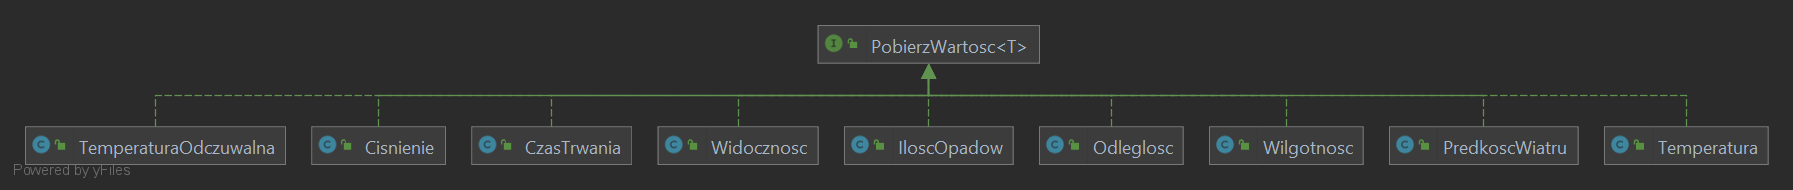
\includegraphics[width=14cm]{uml_2.png}
 \vspace{-0.3cm}
 \caption{Diagram uml pakietu Zmienne. }
 \label{uml_zmienne}
\end{figure}


W programie został zaimplementowany pakiet Zmienne posiadający interfejs PobierzWartosc, k który jest implementowany przez 9 klas reprezentujących analizowane pola z obiektu Wypadek. 

\newpage

%%%%%%%%%%%%%%%%%%%%%%%%%%%%%%%%%%%%%%%%%%%%%%%

\subsection{Diagram UML generatora podsumowań. Krótka instrukcja użytkownika} 

\subsubsection{Diagram UML}

\begin{figure}[h!]
 \centering
 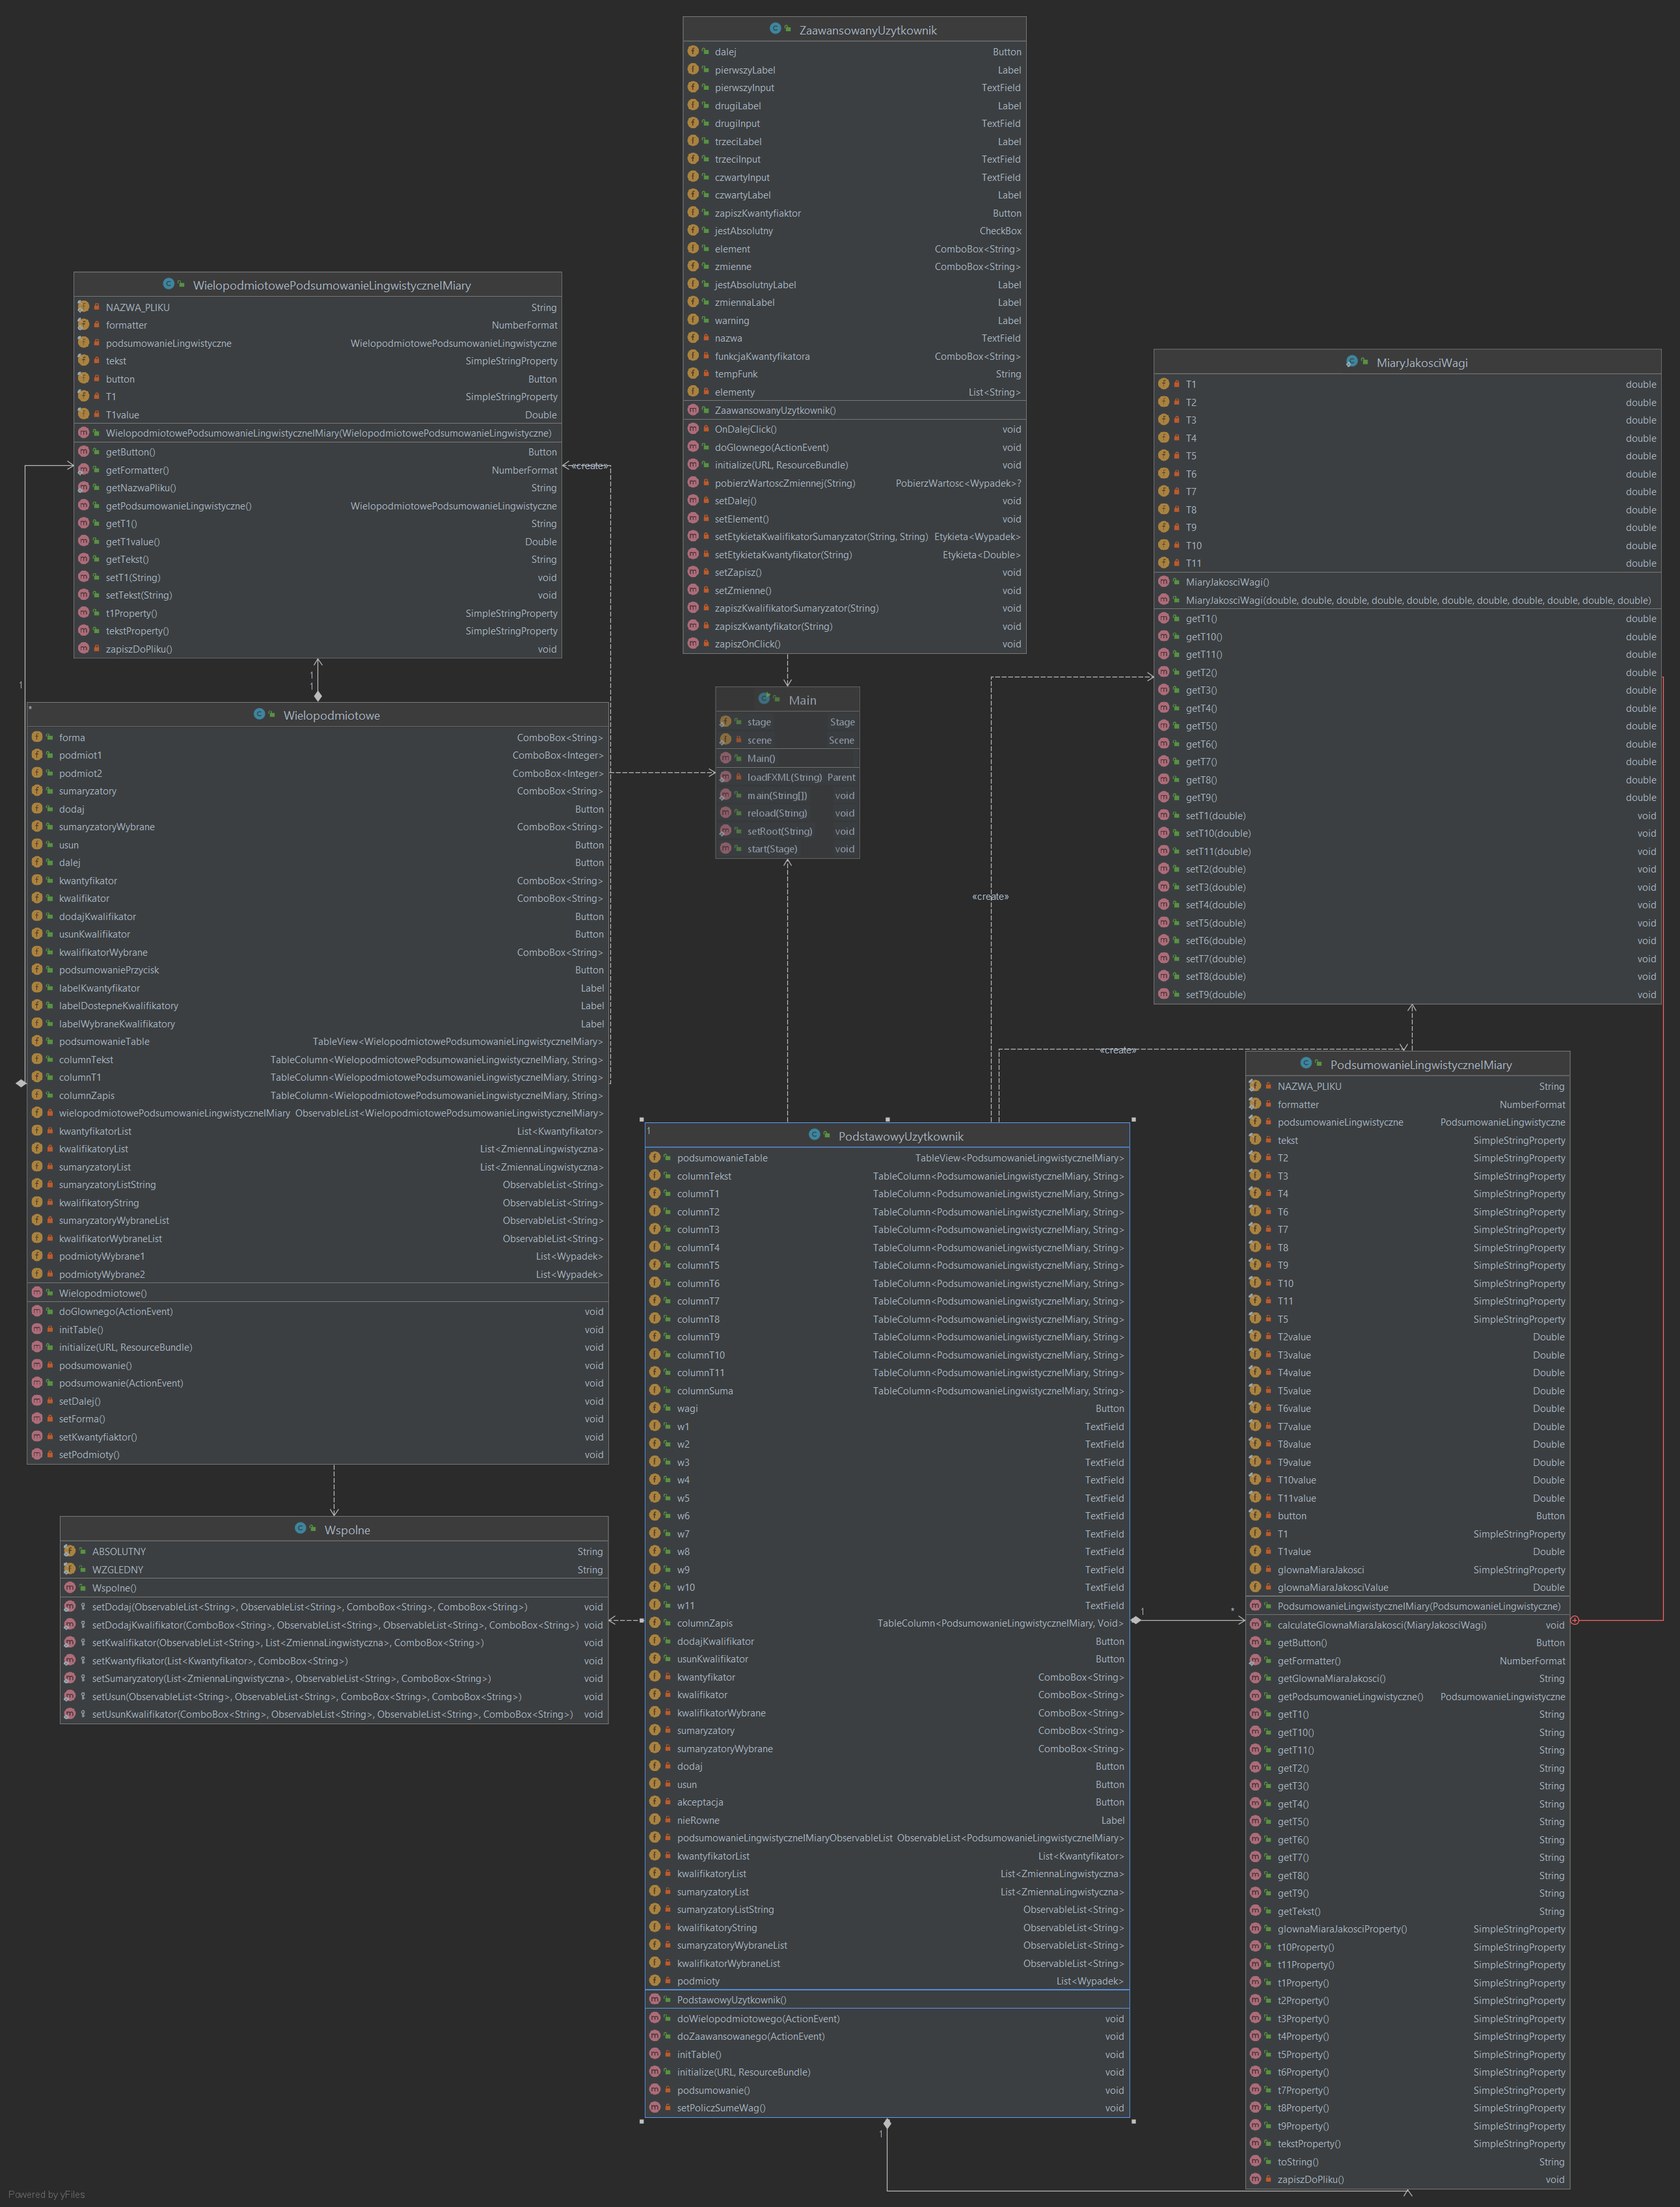
\includegraphics[width=15cm]{uml_3.png}
 \vspace{-0.3cm}
 \caption{Diagram uml interfejsu użytkownika }
 \label{uml_gui}
\end{figure}

W celu stworzenia GUI zostały stworzone dwa pakiety gui oraz predefiniowany. Jedną z dwóch klas znajdujących się w pakiecie predefiniowane jest klasa PredefiniowaneKwantyfiaktory. Jest to klasa reprezentująca singleton, zawiera listę predefiniowanych kwantyfikatorów oraz metodę zwracająca wspomnianą listę. Posiada również metodę pozwalająca na dodanie kwantyfikatora do listy, która jest wykorzystywana, gdy użytkownik zaawansowany dodaje własny kwantyfiaktor. Drugą klasą w wymienionym pakiecie jest klasa PredefiniowaneKwalifikatorySumaryzatory, która również jest klasą reprezentującą singleton. Zawiera pola będące zmiennymi lingwistycznymi dla każdego z atrybutów wypadku, a także metody zwracające każdą ze zmiennych, bądź wszystkie zmienne w liście. Klasa zawiera metody pozwalające na dodanie kwalifikatorów lub sumaryzatorów do listy, która jest wykorzystywana, gdy użytkownik zaawansowany dodaje własny kwalifikator lub sumaryzator. W pakiecie gui znajduje się klasa PodstawowyUzytkownik, która jest kontrolerem łączącym się z oknem wyświetlanym użytkownikowi. Znajdują się w niej pola reprezentujące elementy wyświetlane w interfejsie użytkownika oraz niezbędne listy zmiennych lingwistycznych bądź Stringów, zawierające elementy do wyświetlenia w interfejsie użytkownika. Klasa posiada również metody służące wybraniu wskazanych kwantyfikatorów, kwalifikatorów oraz sumaryzatorów w celu wykonania podsumowania lingwistycznego. Klasa zawiera metodę doZaawansowanego, która otwiera okno dla zaawansowanego użytkownika. Klasa, do generowania podsumowania lignwistycznego wykorzystuje klasę MiaryJakosciWagi oraz PodsumowanieLingwistyczneIMiary. Klasa MiaryJakosciWagi zawiera pola zaiwerające warotści wag dla poszczególnych miar jakości. Klasa 
PodsumowanieLingwistyczneIMiary zawiera metodę getGlownaMiaraJakosci zwracającą w postaci Stringa wartość głównej miary jakości na podstawie wag miar jakości oraz warotści miar jakości. W celu obliczenia głownej miary jakości konstruktor klasy wykorzystuje metodę calculateGlownaMiaraJakosci, która oblicza wspomnianą miarę. W pakiecie gui znajduje się również klasa ZaawansowanyUzytkownik, będąca kontrolerem, w której znajdują się pola dla każdego z elementów wyświetlanych w interfejsie użytkownika. Klasa pozwala na definiowanie własnych kwantyfikatorów, kwalifikatorów i sumaryzatorów. Metody setEtykietaKWantyfikator oraz setEtykietaKwalifikatorSumaryzator pozwalają na stworzenie obiektu Etykieta odpowiednio dla kwantyfiaktora, kwalifikatora lub sumaryzatora. Metody zapiszKwantyfiaktor oraz zapiszKwalifikatorSumaryzator pozwalają na zapis odpwiednio kwantyfiaktora, kwalifikatora lub sumaryzatora do listy dostępnych dla użytkownika kwantyfiaktorów, kwalifikatorów oraz sumaryzatorów. Klasa zawiera metodę doGlownego, która otwiera okno dla podstawowego użytkownika. W pakiecie gui znajduje się klasa Wielopodomiotowe, która jest kontrolerem łączącym się z oknem wyświetlanym użytkownikowi dla generowania wielopodmiotowgo podsumowania lingwistycznego. Znajdują się w niej niezbędne pola reprezentujące elementy wyświetlane w interfejsie użytkownika oraz niezbędne listy zmiennych. Klasa posiada również metody służące pobraniu wartości kwantyfikatorów, kwalifikatorów oraz sumaryzatorów w celu wykonania podsumowania lingwistycznego. Klasa zawiera metodę doGlownego, która otwiera okno dla podstawowego użytkownika. Klasa, do generowania wielopodmiotowych podsumowan lignwistycznych wykorzystuje klasę MiaryJakosciWagi oraz WielopodmiotowePodsumowanieLingwistyczneIMiary. WielopodmiotowePodsumowanieLingwistyczneIMiary to klasa, zaweirajaca metody pozwalające obliczyć miarę jakości \textit{T\textsubscript{1}} dla podsumowań wielopodmiotowych lub zapis do pliku. Klasa PodstawowyUzytkownik oraz Wielopodomiotowe korzystają z klasy Wspolne, która zaiwera metody ustawiające wartości pól wyświetlanych w interfejsie graficznym. 


\newpage


%%%%%%%%%%%%%%%%%%%%%%%%%%%%%%%%%%%%%%%%%%%%%%%
\subsubsection{Instrukcja obsługi}

\begin{figure}[h!]
 \centering
 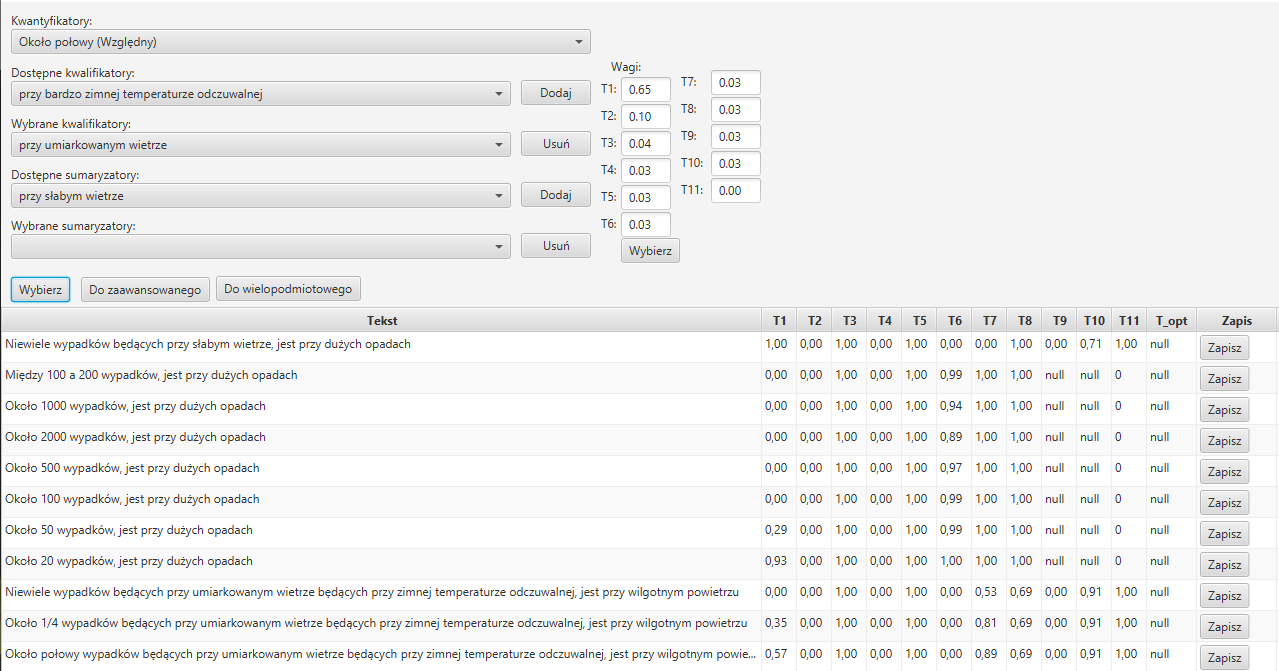
\includegraphics[width=15cm]{gui.png}
 \vspace{-0.3cm}
 \caption{Przykład wyglądu interfejsu podstawowego użytkownika}
 \label{gui}
\end{figure}

Na rysunku \ref{gui}. został przedstawiony podstawowy wygląd interfejsu użytkownika. Zaczynając od lewego górnego roku najpierw użytkownik z rozwijanej listy wybiera kwantyfikator. Następnie z rozwijanej listy wybierany jest jeden bądź wiecej kwalifikatorów, w tym celu użytkownik wybiera pierwszy wybrany kwalifikator i naciska przycisk Dodaj znajdujący się po prawej stronie od rozwijanej listy kwalifikatorów, za pomocą którego wybrany kwalifikator jest dodawany do listy wybranych przez użytkownika kwalifikatorów. Aby wybrać więcej niż jeden kwalifikator użytkownik musi powtórzyć wcześniejsze czynności zaczynając od wybrania z rozwijanej listy pożądanego kwalifikatora. Istnieje możliwość usunięcia kwalifikatora z lsity wybranych kwalifikatorów, w tym celu użytkownik wybiera z rozwijanej listy, znajdującej się pod dostępnymi kwalifikatorami, kwalifikator do usunięcia. Następnie przcyiska przycisk Usuń. W celu usunięcia więcej niż jednego kwalifikatora, użytkownik musi powtórzyć opisane czynności zaczynając od wyboru kwalifikatora z listy wybranych kwalifikatorów. Kolejnym krokiem jest wybranie jednego bądź wielu sumaryzatorów w sposób identyczny do opisanego sposobu wyboru i usuwania kwalifikatorów. W celu wykonania podsumowania lignwistycznego należy przycisnąć przycisk Wybierz znajdujący się pod rozwijaną listą z wybranymi sumaryzatorami, następnie w tabeli na dole ekranu pojawi się wygenerowany tekst podsumowania oraz wartości miar jakości. W ostatniej kolumnie tabeli znajduje sie przycisk Zapisz, dla każdego wygenerowanego podsumwoania. Po przyciśnięciu opisanego przycisku dane podsumowanie zostanie dopisane do pliku txt. W programie istnieje możliwość obliczenia głównej miary podsumowania, w tym celu należy wpisać odpowiednie wagi, dla każdej z miar w polach znajdujących się na środku ekranu. Pod polami znajduje się przycisk Wybierz, którego kliknięcie spowoduje policzenie głównej miary podsumowań we wszystkich podsumowaniach znajdujących się w tabeli. Kliknięcie przycisku Do zaawansowanego spowoduje przejście do ekranu użytkownika zaawansowanego. Kliknięcie przycisku Do wielopodmiotowego spowoduje przejście do ekranu wielopodmiotowych podsumowań lingwistycznych. 

\begin{figure}[h!]
 \centering
 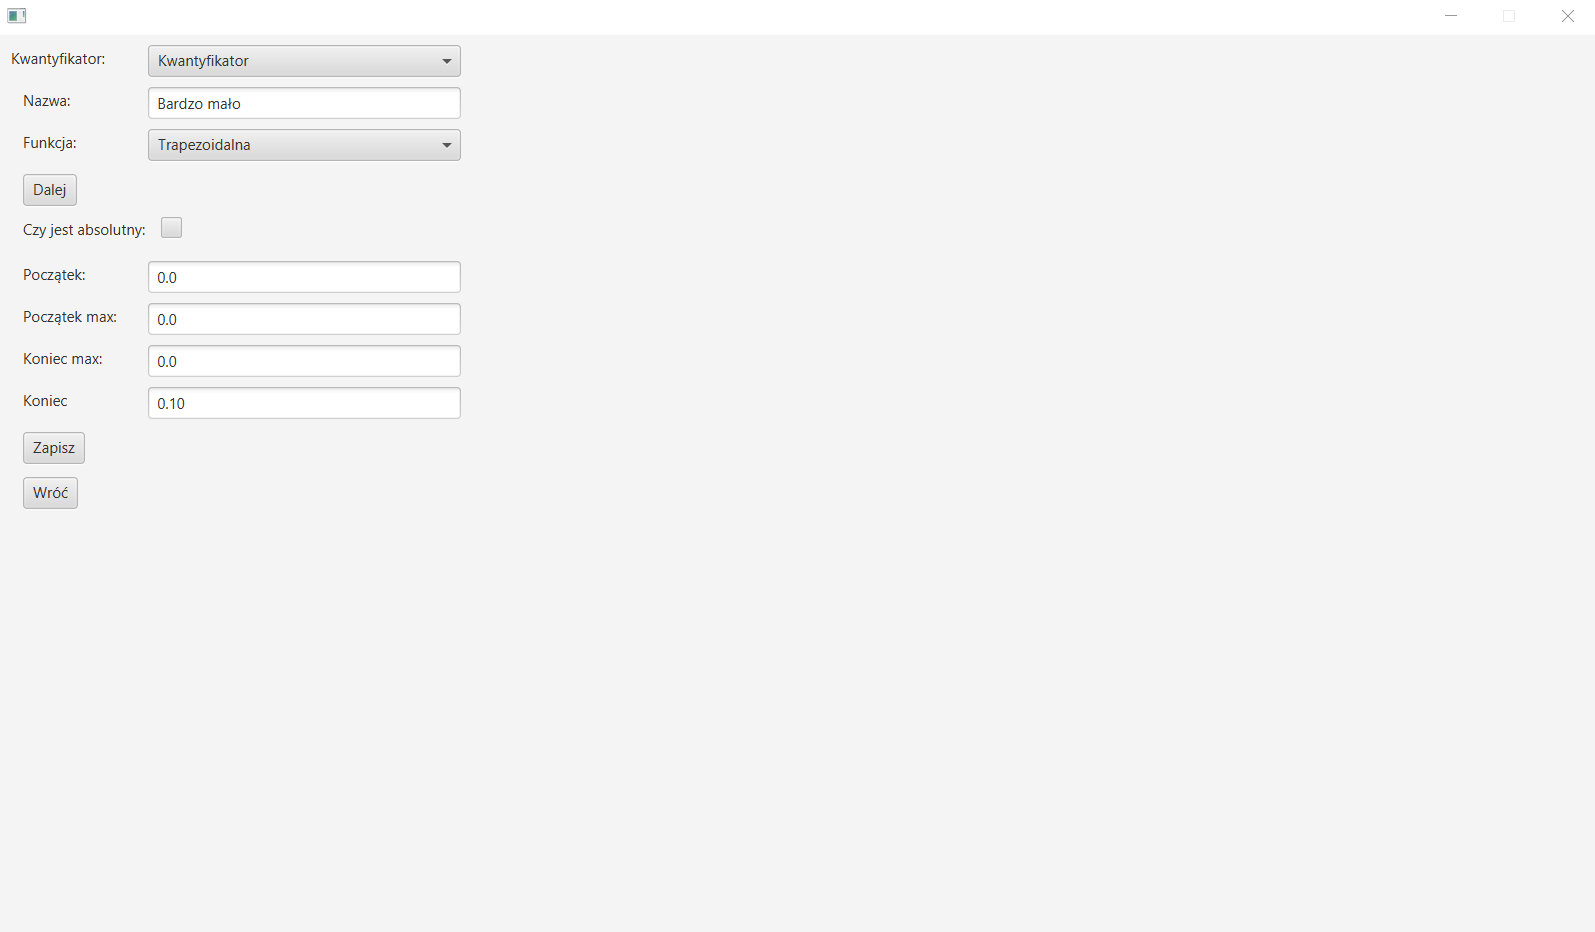
\includegraphics[width=15cm]{gui_2.png}
 \vspace{-0.3cm}
 \caption{Przykład wyglądu interfejsu zaawansowanego użytkownika}
 \label{gui2}
\end{figure}

Na rysunku \ref{gui2}. został przedstawiony wygląd interfejsu zaawansowanego użytkownika, który służy do tworzenia własnych kwantyfikatorów, klasyfikatorów oraz sumaryzatorów. Zaczynając od lewego górnego rogu na użytkownik wybiera, który z elementów chce utworzyć: kwantyfiaktor, kwalifikator, sumaryzator. Następnie poniżej należy wpisać nazwę elementu oraz wybrać z rozwijanej listy funkcję przynależności. Kliknięcie przcisku Dalej powoduje pojawienie się pól do wprowadzenia kolejnych danych w zależności od cześniej wybranych wartości. Dla warotści wybranych na rysunku \ref{gui2} po kliknięciu przyciski Dalej pojawią się następujące pola: checkbox do zaznaczenia czy kwantyfiaktor jest absolutny, początek funkcji przynależności, początek i koniec maksymalnej wartości, dla których funkcja przyjmuje wartość maksymalną oraz wartość końcową. Kliknięcie przycisku Zapisz spowosuje zapisanie elementu do listy dostępnych elementów. Przyciśnięcie przycisku Wróć wróci do ekranu użytkownika podstawowego. \\

\begin{figure}[h!]
 \centering
 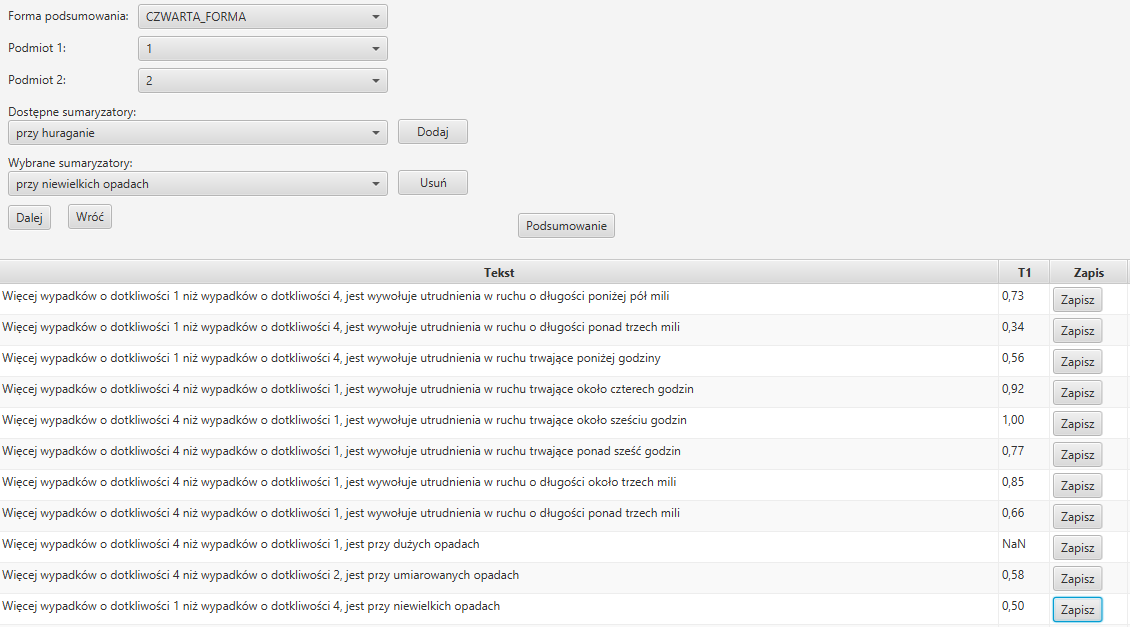
\includegraphics[width=15cm]{gui_3.png}
 \vspace{-0.3cm}
 \caption{Przykład wyglądu interfejsu zaawansowanego użytkownika}
 \label{gui3}
\end{figure}

\newpage

Na rysunku \ref{gui3}. został przedstawiony wygląd interfejsu użytkownika dla generowania wielopodmiotowych podsumowań lingwistycznych. Zaczynając od góry użytkownik wybiera z rozwijanej listy formę podsumowania lingwistycznego, następnie wybiera dla podmiotu 1 i 2 typ podmiotów, dostępne są wypadki o dotkliwości 1, 2, 3 bądź 4. W kolejnym kroku wybiera sumaryzator zgodnie z instrukcja dla interfejsu użytkownika podstawowego. Kliknięcie przycisku dalej powoduje pokazanie się ewentualnych pól do uzupełnienia w zależności od formy podsumowania, która została wybrana. Pola, które mogą się pojawić to kwantyfiaktor oraz kwalifikator. Kliknięcie przycisku Podsumowanie powoduje wygenerownanie wielopodmiotowego posumowania lingwistycznego. 


Wymagania, które muszą zostać spełnione by uruchomić program na własnym komputerze to: wersja Javy 11. 

\newpage




%%%%%%%%%%%%%%%%%%%%%%%%%%%%%%%%%%%%%%%%%%%%%%%
\section{ Jednopodmiotowe podsumowania lingwistyczne. Miary jakości, podsumowanie optymalne}
\label{section:ex}
\subsection{Eksperyment 1}
\label{section:ex1}
\begin{figure}[h!]
 \centering
 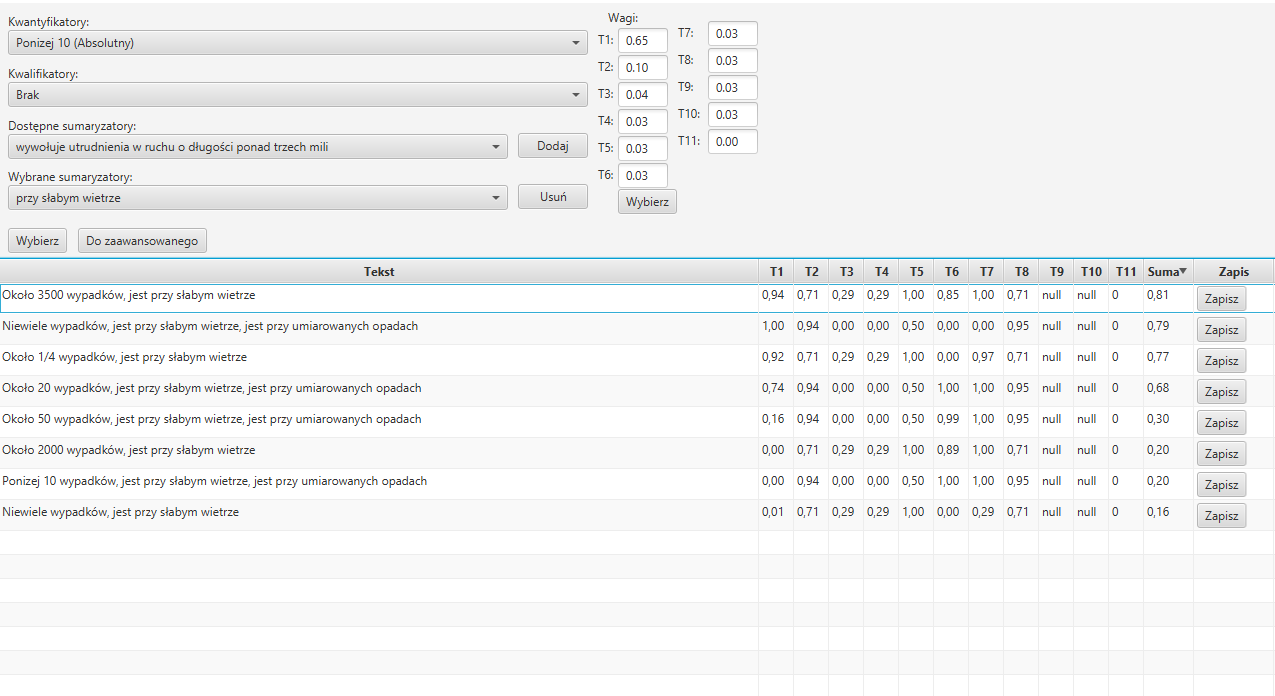
\includegraphics[width=15cm]{ex1.png}
 \vspace{-0.3cm}
 \caption{Tabela przedstawia wyniki podsumowań lingwistycznych dla eksperymentu 1. Kolumna Tekst zawiera tekst wygenerowanego podsumowania lingwistycznego. Kolumny T\textsubscript{1}-T\textsubscript{11} są miarami jakości podsumowania lignwistycznego \cite{niewiadomski19}. Kolumna T\textsubscript{opt} zawiera wartości jakości optymalnego podsumowania lingwistycznego, które są średnią ważoną miar jakości od \textit{T\textsubscript{1}} do \textit{T\textsubscript{11}}. Ostatnia kolumna, Zapisz, zawiera przcisk zapisujący dane podsumwoanie lignwistyczne do pliku. Każdy rząd zawiera jedno wygenerowane podsumowanie lignwistyczne. Rzędy zostały posortowane po kolumnie T\textsubscript{opt} malejąco. }
 \label{ex1}
\end{figure}

W pierwszym eksperymencie wygenerowaliśmy jednopodmiotowe podsumowania lingwistyczne w pierwszej formie. Do obliczenia miary jakości podsumowania optymalnego zostały użyte następujące wagi odpowiednio dla miar od \textit{T\textsubscript{1}} do \textit{T\textsubscript{11}}: 0.65, 0.10, 0.04, 0.03, 0.03, 0.03, 0.03, 0.03, 0.03, 0.03, 0.00. 

Na podstawie tabeli \ref{ex1} można zauważyć, że zdanie "Niewiele wypadków, jest przy słabym wietrze, jest przy umiarkowanych opadach [0.79]" jest zdaniem najbardziej zgodnym z prawdą dla kwantfikatorów względnych, ponieważ nie ma wielu wypadków, które były przy słabym wietrze i umiarkowanych opadach. Natomiast patrząc na zdanie, które jest najmniej zgodne z prawdą, "Niewiele wypadków, jest przy słabym wietrze [0.16]", wnioskujemy, że jest wiele wypadków, które nastąpiły przy słabym wietrze. Zdanie "Około 3500 wypadków, jest przy słabym wietrze [0.81]" jest zdaniem najbardziej zgodnym z prawdą. 


%%%%%%%%%%%%%%%%%%%%%%%%%%%%%%%%%%%%%%%%%%%%%%%
\newpage
\subsection{Eksperyment 2}
\label{section:ex2}
\begin{figure}[h!]
 \centering
 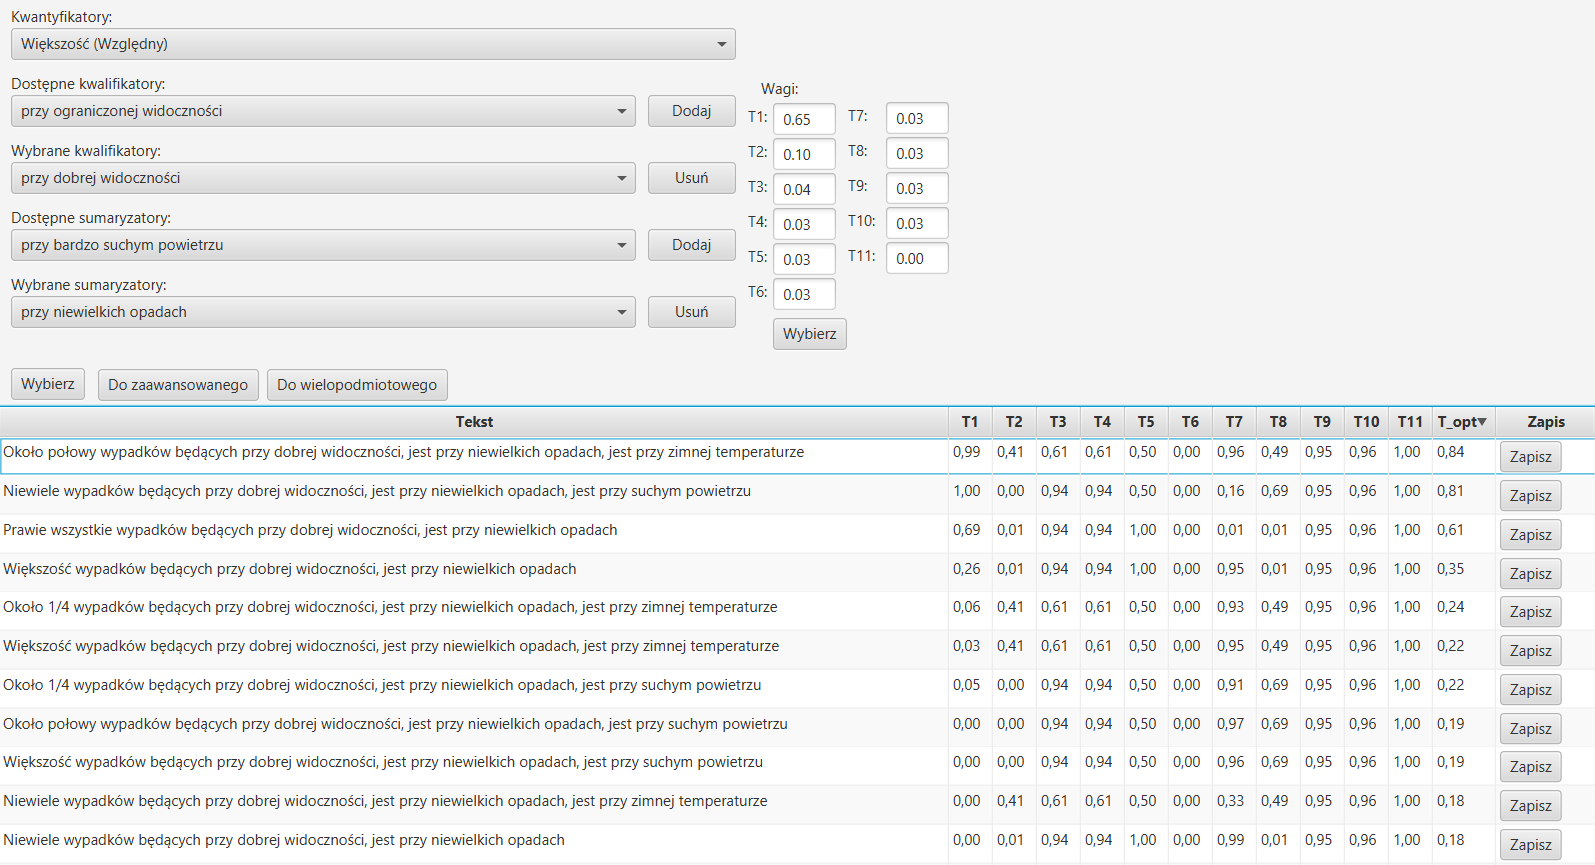
\includegraphics[width=15cm]{ex2.png}
 \vspace{-0.3cm}
 \caption{Tabela przedstawia wyniki podsumowań lingwistycznych dla eksperymentu 2. Kolumna Tekst zawiera tekst wygenerowanego podsumowania lingwistycznego. Kolumny T\textsubscript{1}-T\textsubscript{11} są miarami jakości podsumowania lignwistycznego \cite{niewiadomski19}. Kolumna T\textsubscript{opt} zawiera wartości jakości optymalnego podsumowania lingwistycznego, które są średnią ważoną miar jakości od \textit{T\textsubscript{1}} do \textit{T\textsubscript{11}}. Ostatnia kolumna, Zapisz, zawiera przcisk zapisujący dane podsumwoanie lignwistyczne do pliku. Każdy rząd zawiera jedno wygenerowane podsumowanie lignwistyczne. Rzędy zostały posortowane po kolumnie T\textsubscript{opt} malejąco. }
 \label{ex2}
\end{figure}

W drugim eksperymencie wygenerowaliśmy jednopodmiotowe podsumowania lingwistyczne w drugiej formie. Do obliczenia miary jakości podsumowania optymalnego zostały użyte następujące wagi odpowiednio dla mair od \textit{T\textsubscript{1}} do \textit{T\textsubscript{11}}: 0.65, 0.10, 0.04, 0.03, 0.03, 0.03, 0.03, 0.03, 0.03, 0.03, 0.00. 

Na podstawie tabeli \ref{ex2} można zauważyć, że zdanie "Około połowy wypadków będących przy  dobrej widoczności, jest przy niewielkich opadach, jest przy zimnej temperaturze [0.84]" jest zdaniem najbardziej zgodnym z prawdą, a jednocześnie zdanie "Niewiele wypadków będących przy  dobrej widoczności, jest przy niewielkich opadach, jest przy zimnej temperaturze [0.18]" jest zdaniem najmniej zgodnym z prawdą. Można zauważyć, że te zdania zaprzeczają sobie nazwajem, więc wyniki miar jakości podsumowania optymalnego są uzasadnione. Zgodnie z naszymi oczekiwaniami "Prawie wszystkie wypadki będące przy dobrej widoczności, jest przy niewielkich opadach [0.61]", jest trzecim zdaniem najbardziej zgodnym z prawdą, ponieważ opady powodują złą widoczność, więc jeśli widoczność była dobra oznacza to, że opadów nie było, bądź były niewielkie. Natomaist zdanie "Niewiele wypadków będących przy dobrej widoczności, jest przy niewielkich opadach, jest przy suchym powietrzu [0.18]" nie było zgodne z naszymi oczekiwaniami, ponieważ spodziewaliśmy się, że przy większości wypadków jeśeli jest dobra widoczność, to nie ma opadów, a co za tym idzie jest suche powietrze, co okazało się być zdaniem nieprawdziwym. 

%%%%%%%%%%%%%%%%%%%%%%%%%%%%%%%%%%%%%%%%%%%%%%%
\newpage
\subsection{Eksperyment 3}
\label{section:ex3}
\begin{figure}[h!]
 \centering
 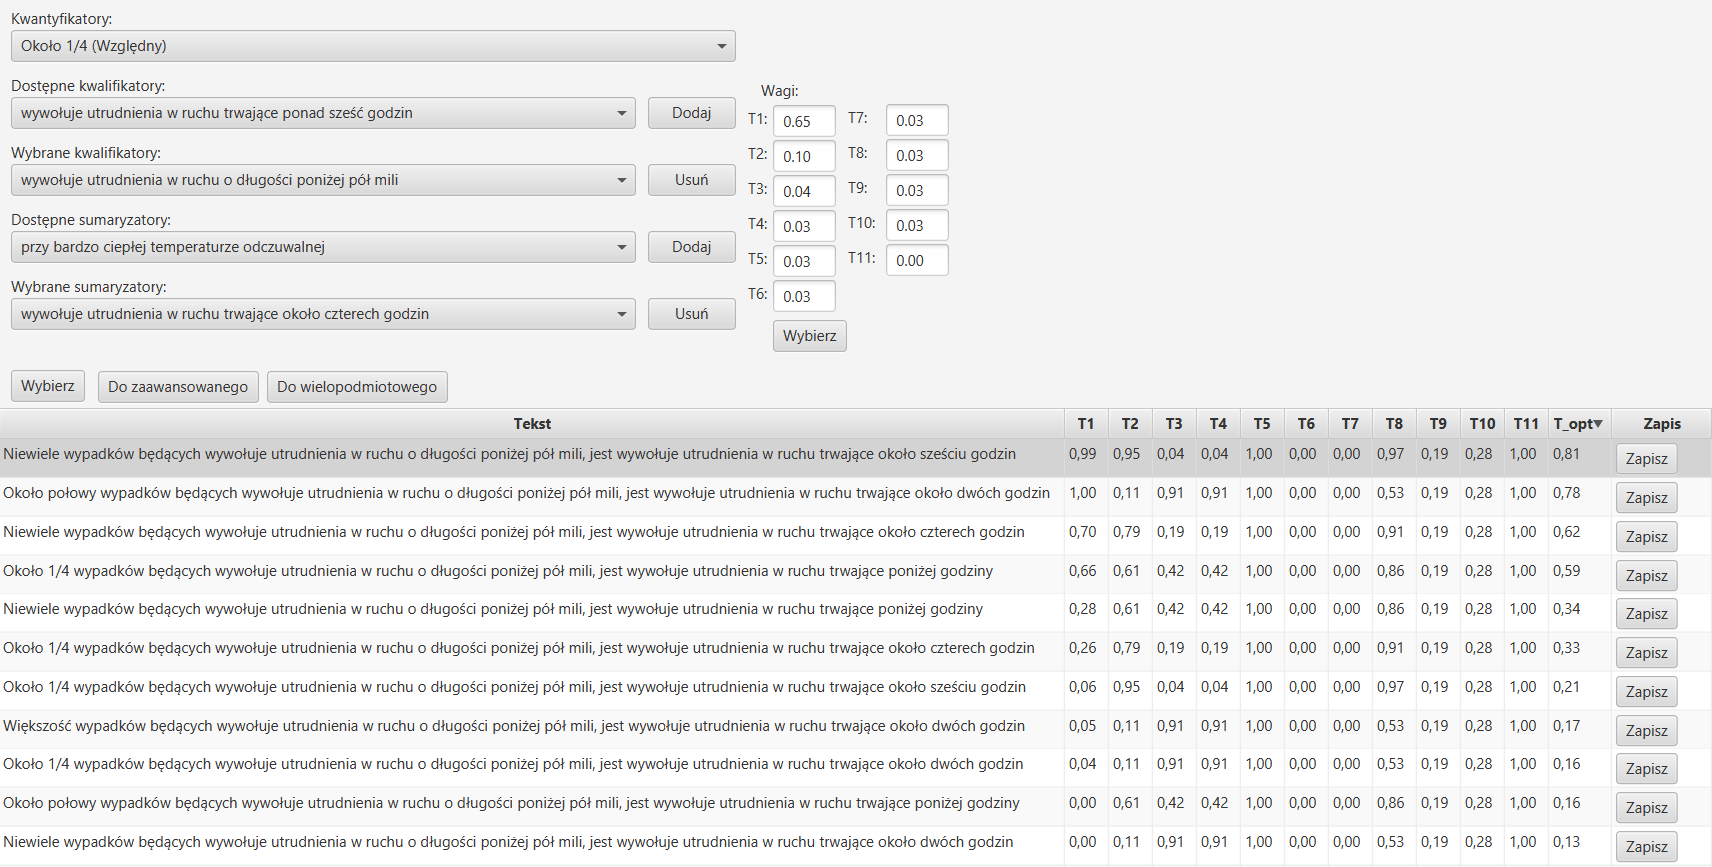
\includegraphics[width=15cm]{ex3.png}
 \vspace{-0.3cm}
 \caption{Tabela przedstawia wyniki podsumowań lingwistycznych dla eksperymentu 3. Kolumna Tekst zawiera tekst wygenerowanego podsumowania lingwistycznego. Kolumny T\textsubscript{1}-T\textsubscript{11} są miarami jakości podsumowania lignwistycznego \cite{niewiadomski19}. Kolumna T\textsubscript{opt} zawiera wartości jakości optymalnego podsumowania lingwistycznego, które są średnią ważoną miar jakości od \textit{T\textsubscript{1}} do \textit{T\textsubscript{11}}. Ostatnia kolumna, Zapisz, zawiera przcisk zapisujący dane podsumwoanie lignwistyczne do pliku. Każdy rząd zawiera jedno wygenerowane podsumowanie lignwistyczne. Rzędy zostały posortowane po kolumnie T\textsubscript{opt} malejąco.  }
 \label{ex3}
\end{figure}

W trzecim eksperymencie wygenerowaliśmy jednopodmiotowe podsumowania lingwistyczne w drugiej formie. Do obliczenia miary jakości podsumowania optymalnego zostały użyte następujące wagi odpowiednio dla mair od \textit{T\textsubscript{1}} do \textit{T\textsubscript{11}}: 0.65, 0.10, 0.04, 0.03, 0.03, 0.03, 0.03, 0.03, 0.03, 0.03, 0.00. 

Wykonany eksperyment miał na celu sprawdzenie zależności długości odcinka drogi, na którym nastąpiły utrudnienia w ruchu spowodowane przez wypadek od czasu trwania utrudnień w ruchu drogowym przez ten wypadek. Uzyskane wyniki potwierdzają postawioną tezę. Na podstawie tabeli \ref{ex3} można zauważyć, że zdanie "Około połowy wypadków będących wywołuje utrudnienia w ruchu o długości poniżej pół mili, jest wywołuje utrudnienia w ruchu trwające około dwóch godzin [0.81]" jest najbardziej prawdziwym zdaniem. Jednocześnie możemy zauważyć, że to samo zdanie z kwantyfiaktorem "Niewiele" jest najmniej prawdziwym zdaniem. To samo zdanie z kwantyfiaktorami "Około 1/4" lub "Większość" są zdecydowanie mniej prawdziwe niż pierwsze opisane zdanie. Kolejnym zdaniem potwierdzającym tezę jest: "Niewiele wypadków będących wywołuje utrudnienia w ruchu o długości poniżej pół mili, jest wywołuje utrudnienia w ruchu trwające około sześciu godzin [0.81]", ponieważ, odcinek poniżej pół mili jest krótkim odcinkiem, a czas trwania sześć godzin jest znacznie długim czasem. Ze zdania możemy odczytać, że nie wiele wypadków będących na krótkim odcinku drogi wywoluje tak długi czas trwania utrudnień w ruchu drogowym.


%%%%%%%%%%%%%%%%%%%%%%%%%%%%%%%%%%%%%%%%%%%%%%%
\section{Wielopodmiotowe podsumowania lingwistyczne i~ich miary jakości} 
\label{section:ex_wiel}

Zbiór danych został podzielony na rozłączne podmioty na podstawie kolumny Dotkliwość (Severity). Kolumna przyjmuje liczby całkowite od 1 do 4 włącznie. Im wyższa wartość kolumny tym bardziej dotkliwy był wypadek. W ten sposób uzyskujemy 4 rozłączne podzbiory podmiotów, które są podzielone ze względu na wpływ wypadku na ruch drogowy, gdzie wartość kolumny 1 oznacza najmniejszy wpływ, natoamist wartość 4 największy wpływ wypadku na ruch drogowy. 

%%%%%%%%%%%%%%%%%%%%%%%%%%%%%%%%%%%%%%%%%%%%%%%

\subsection{Eksperyment 1}
\label{section:ex_wiel1}

\begin{figure}[h!]
 \centering
 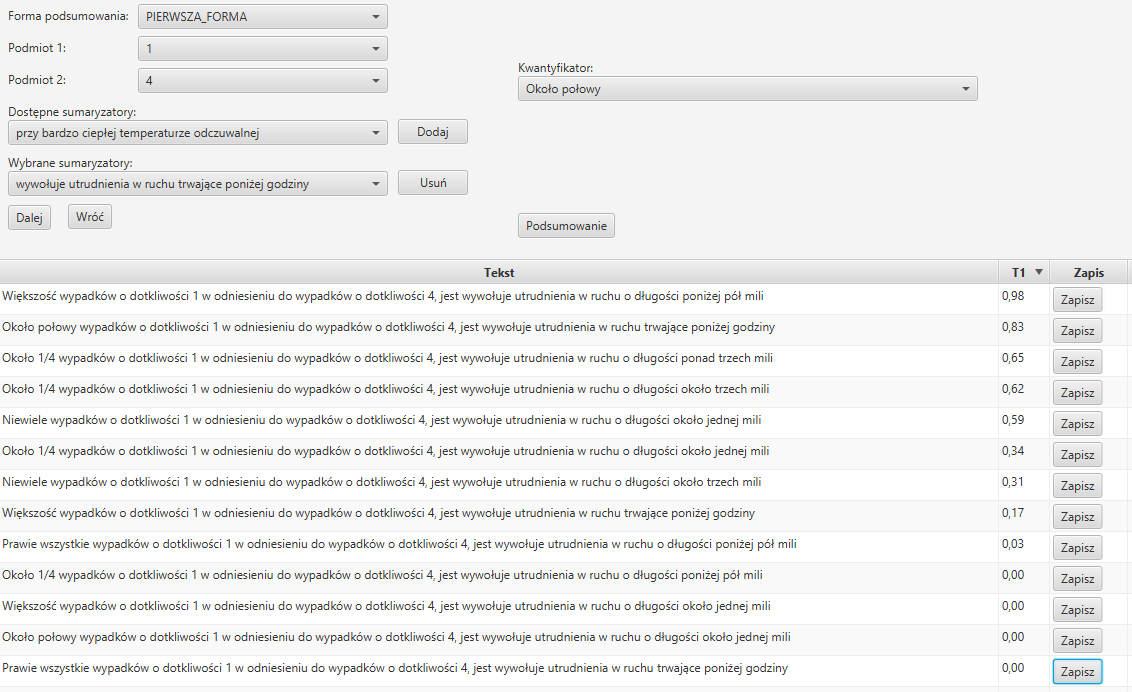
\includegraphics[width=15cm]{ex_wiel1.png}
 \vspace{-0.3cm}
 \caption{Tabela przedstawia wyniki wielopodmiotowych podsumowań lingwistycznych w pierwszej formie dla eksperymentu 1. Kolumna Tekst zawiera tekst wygenerowanego wielopodmiotowego podsumowania lingwistycznego. Kolumna \textit{T\textsubscript{1}} zawiera wartość miary jakości \textit{T\textsubscript{1}} dla wielopodmiotowego podsumowania lignwistycznego \cite{niewiadomski19}. Ostatnia kolumna, Zapisz, zawiera przcisk zapisujący dane wielopodmiotowego podsumowania lignwistycznego do pliku. Każdy rząd zawiera jedno wygenerowane wielopodmiotowe podsumowanie lignwistyczne. Rzędy zostały posortowane po kolumnie \textit{T\textsubscript{1}} malejąco.  }
 \label{wykr_ex_wiel1}
\end{figure}
\newpage

W pierwszym eksperymencie wygenerowaliśmy wielopodmiotowe podsumowania lingwistyczne w pierwszej formie. 

Na podstawie tabeli z Rysunku \ref{wykr_ex_wiel1} można zauważyć, że zdanie "Większość wypadków o dotkliwości 1 w odniesieniu do wypadków o dotkliwości 4, jest wywołuje utrudnienia w ruchu o długości poniżej pół mili [0.98]" jest zdaniem najbardziej zgodnym z prawdą z wszystkich wygenerowanych podsumowań wielopodmiotowych. Zgodnie z naszymi oczekiwaniami, zdecydowanie więcej wypadków o dotkliwości 1 (mających najmniejszy wpływ na ruch drogowy) wywoływało utrudunienia w ruchu o długości poniżej pół mili, czyli utrudnienia na najmniejszym odcinku drogi, w porównaniu do wypadków o dotkliwości 4 (majacych największy wpływ na ruch drogowy).  Zdanie "Około 1/4 wypadków o dotkliwości 1 w odniesieniu do wypadków o dotkliwości 4, jest wywołuje utrudnienia w ruchu o długości ponad trzech mili [0.65]" jest trzecim wygenerowanym podsumowaniem najbardziej zgodnym z prawdą. Wspomniane zdanie również jest zgodne z naszymi oczekiwaniami, ponieważ zdecydowanie mniej wypadków o dotkliwości 1  w porównaniu do wypadków o dotkliwości 4 wywłuje utrudnienia w ruchu drogowym o długości ponad 3 mln, czyli najdłuższe utrudnienia. Z tego zdania wynika, że większość wypadków powodujących najdłuższe utrudnienia w ruchu drogowym są o największej dotkliwości, z pierwszego opisanego w tym eksperymencie zdania wynika, że najkrótsze utrudnienia w ruchu drogowym powodują wypadki o najmniejszej dotkliwości. 

%%%%%%%%%%%%%%%%%%%%%%%%%%%%%%%%%%%%%%%%%%%%%%%
\newpage
\subsection{Eksperyment 2}
\label{section:ex_wiel2}

\begin{figure}[h!]
 \centering
 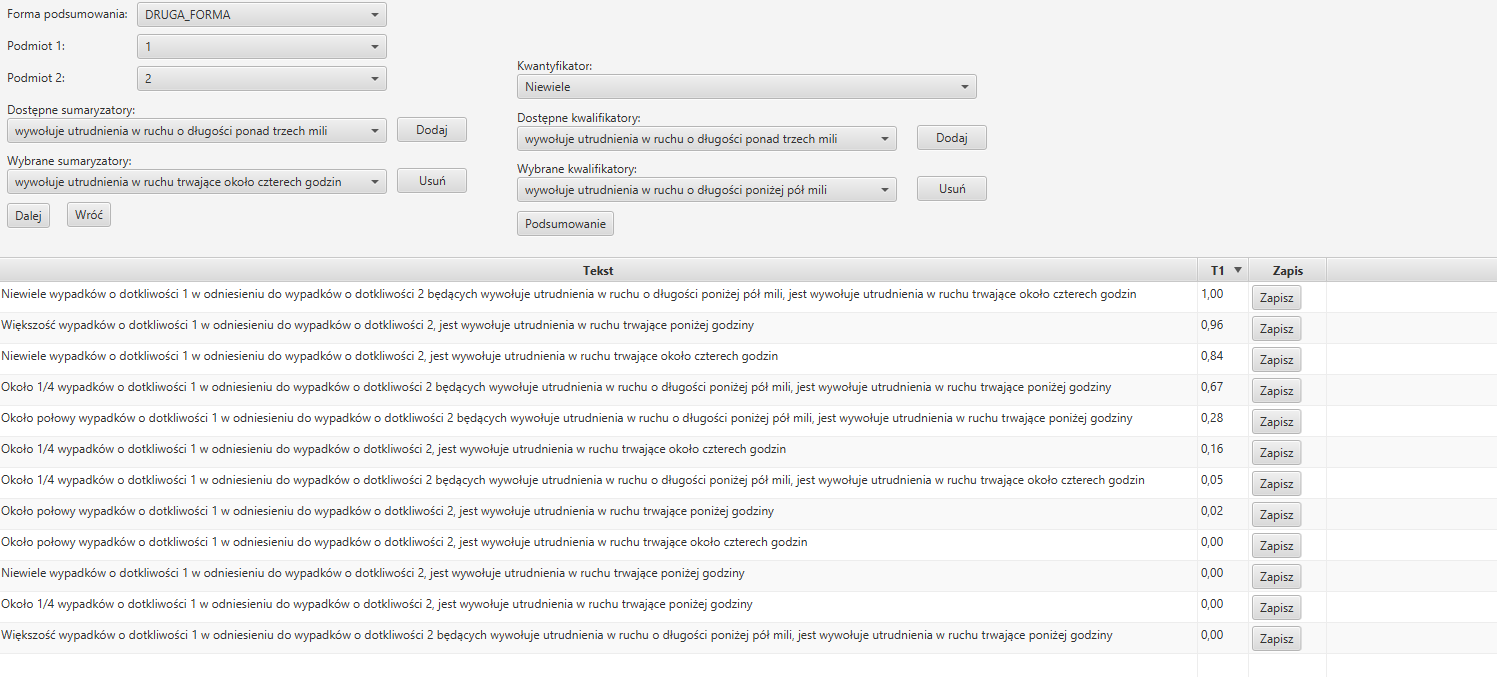
\includegraphics[width=15cm]{ex_wiel2.png}
 \vspace{-0.3cm}
 \caption{Tabela przedstawia wyniki wielopodmiotowych podsumowań lingwistycznych w drugiej formie dla eksperymentu 2. Kolumna Tekst zawiera tekst wygenerowanego wielopodmiotowego podsumowania lingwistycznego. Kolumna \textit{T\textsubscript{1}} zawiera wartość miary jakości \textit{T\textsubscript{1}} dla wielopodmiotowego podsumowania lignwistycznego \cite{niewiadomski19}. Ostatnia kolumna, Zapisz, zawiera przcisk zapisujący dane wielopodmiotowego podsumowania lignwistycznego do pliku. Każdy rząd zawiera jedno wygenerowane wielopodmiotowe podsumowanie lignwistyczne. Rzędy zostały posortowane po kolumnie \textit{T\textsubscript{1}} malejąco.  }
 \label{wykr_ex_wiel2}
\end{figure}

W drugim eksperymencie wygenerowaliśmy wielopodmiotowe podsumowania lingwistyczne w pierwszej oraz drugiej formie. 

Na podstawie tabeli z Rysunku \ref{wykr_ex_wiel2} można zauważyć, że zdanie "Większość wypadków o dotkliwości 1 w odniesieniu do wypadków o dotkliwości 2, jest wywołuje utrudnienia w ruchu trwające poniżej godziny [0.96]" jest podumowaniem, które jest najbardziej prawdziwe z wygenerowanych zdań w pierwszej formie. Natomiast możemy zauważyć, że to samo zdnanie w drugiej formie z kwalifikatorem "wywołuje utrudnienia w ruchu o długości ponieżej pół mili" jest zdaniem najmniej prawdziwym. Różnica może być spowodowana, że w drugim zdaniu z wypadków o dotkliwości 2 zostały odjęte wypadki powodujące utrudnienia w ruchu powyżej pół mili. Zostały więc wypadki o dotkliwości 2, które mogły mieć według nas największe szanse na wywołanie utrudnień w ruchu trwających poniżej godziny. 

\newpage

\begin{figure}[h!]
 \centering
 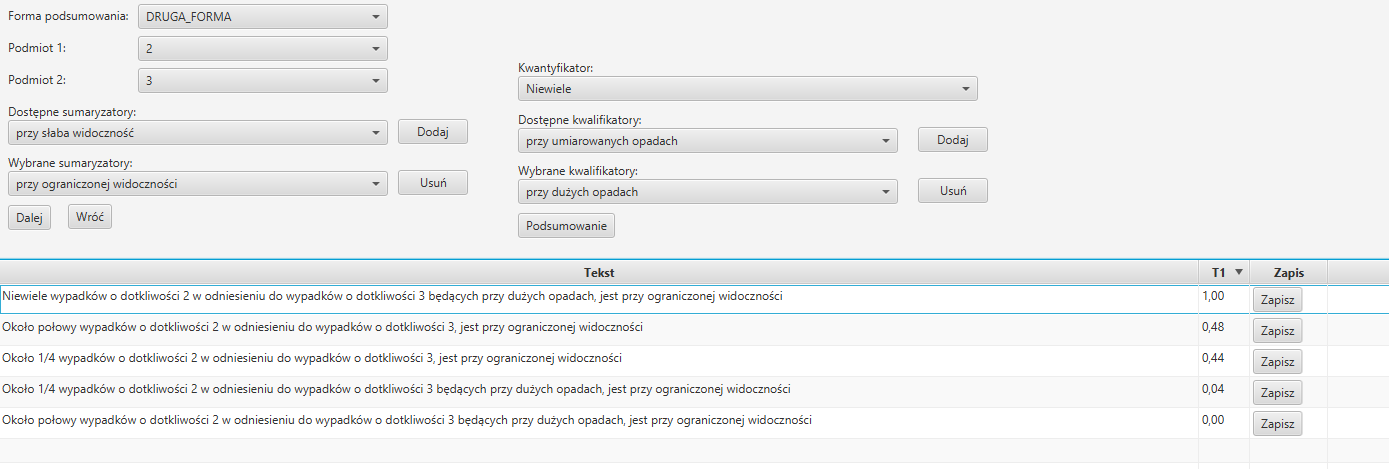
\includegraphics[width=15cm]{ex_wiel2_2.png}
 \vspace{-0.3cm}
 \caption{Tabela przedstawia wyniki wielopodmiotowych podsumowań lingwistycznych w drugiej formie dla eksperymentu 2. Kolumna Tekst zawiera tekst wygenerowanego wielopodmiotowego podsumowania lingwistycznego. Kolumna \textit{T\textsubscript{1}} zawiera wartość miary jakości \textit{T\textsubscript{1}} dla wielopodmiotowego podsumowania lignwistycznego \cite{niewiadomski19}. Ostatnia kolumna, Zapisz, zawiera przcisk zapisujący dane wielopodmiotowego podsumowania lignwistycznego do pliku. Każdy rząd zawiera jedno wygenerowane wielopodmiotowe podsumowanie lignwistyczne. Rzędy zostały posortowane po kolumnie \textit{T\textsubscript{1}} malejąco.  }
 \label{wykr_ex_wiel2_2}
\end{figure}



Na podstawie tabeli z Rysunku \ref{wykr_ex_wiel2_2} można zauważyć, że zdanie "Niewiele wypadków o dotkliwości 2 w odniesieniu do wypadków o dotkliwości 3 będących przy dużych opadach, jest przy ograniczonej widoczności [1.0]" jest podumowaniem, które jest najbardziej prawdziwe z wygenerowanych zdań. Oznacza, że zdecydowanie więcej wypadków o dotkliwości 3 będące przy dużych opadach było przy ograniczonej widoczności niż wypadków o dotkliwości 2. Biorąc pod uwagę zdanie: "Około połowy wypadków o dotkliwości 2 w odniesieniu do wypadków o dotkliwości 3, jest przy ograniczonej widoczności [0.00]" możemy zauważyć, że stosunek liczby wypadków o dotkliwości 2 w odniesieniu do wszystkich rozważanych wypadków wynosi niecałe 0.4. Natomiast po dodaniu kwalifikatora "będące przy dużych opadach" wartość ta zmienia się na 0.0. 





%%%%%%%%%%%%%%%%%%%%%%%%%%%%%%%%%%%%%%%%%%%%%%%
\newpage
\subsection{Eksperyment 3}
\label{section:ex_wiel3}

\begin{figure}[h!]
 \centering
 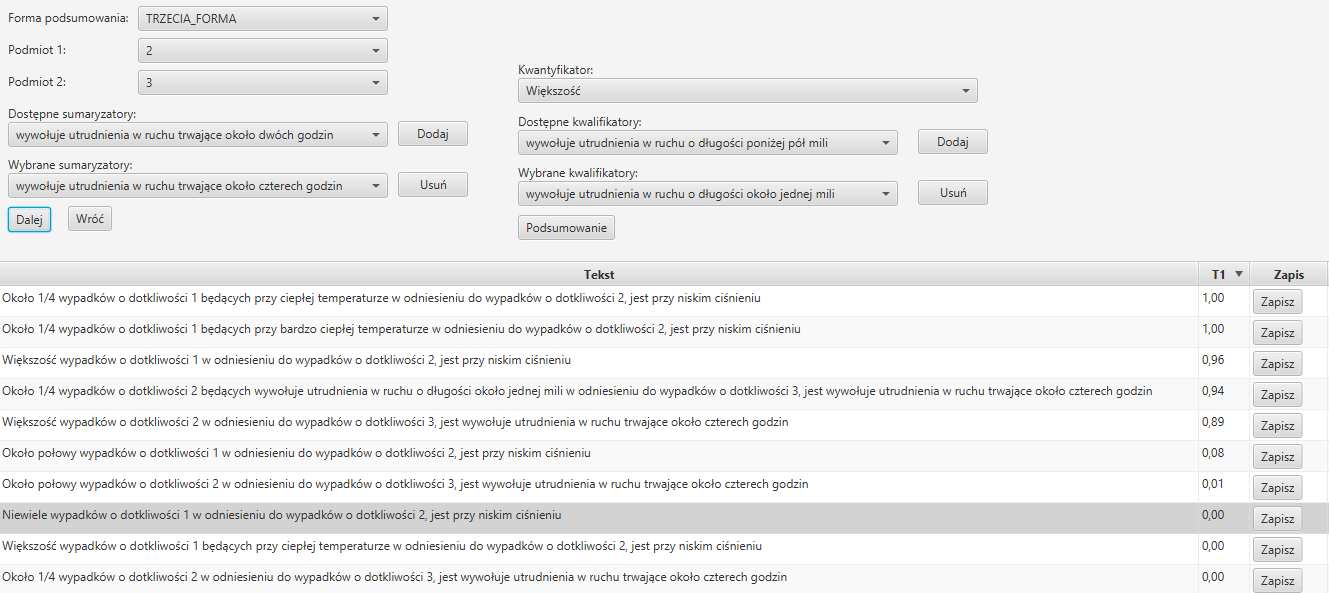
\includegraphics[width=15cm]{ex_wiel3.png}
 \vspace{-0.3cm}
 \caption{Tabela przedstawia wyniki wielopodmiotowych podsumowań lingwistycznych w trzeciej formie dla eksperymentu 3. Kolumna Tekst zawiera tekst wygenerowanego wielopodmiotowego podsumowania lingwistycznego. Kolumna \textit{T\textsubscript{1}} zawiera wartość miary jakości \textit{T\textsubscript{1}} dla wielopodmiotowego podsumowania lignwistycznego \cite{niewiadomski19}. Ostatnia kolumna, Zapisz, zawiera przcisk zapisujący dane wielopodmiotowego podsumowania lignwistycznego do pliku. Każdy rząd zawiera jedno wygenerowane wielopodmiotowe podsumowanie lignwistyczne. Rzędy zostały posortowane po kolumnie \textit{T\textsubscript{1}} malejąco.  }
 \label{wykr_ex_wiel3}
\end{figure}

W trzecim eksperymencie wygenerowaliśmy wielopodmiotowe podsumowania lingwistyczne w pierwszej oraz trzeciej formie. 

Na podstawie tabeli z Rysunku \ref{wykr_ex_wiel3} można zauważyć, że zdanie "Większość wypadków o dotkliwości 1 w odniesieniu do wypadków o dotkliwości 2, jest przy niskim ciśnieniu [0.96]" jest podumowaniem, które ma wysoki stopień prawdziwości i posiada stosunek liczby wypadków o dotkliwości 2 w odniesieniu do wszystkich rozważanych wypadków wynosi około 0.75. Natomiast możemy zauważyć, że to samo zdanie w trzeciej formie z kwalifikatorem "będących przy bardzo ciepłej temperaturze" jest zdaniem najbardziej prawdziwym i stosunek liczby wypadków o dotkliwości 2 w odniesieniu do wszystkich rozważanych wypadków spada do liczby około 0.25. 

Zdanie "Około połowy wypadków o dotkliwości 2 w odniesieniu do wypadków o dotkliwości 3, jest wywołuje utrudnienia w ruchu trwające około czterech godzin [0.01]" jest zdaniem bardzo mało prawdziwym oraz posiada stosunek liczby wypadków o dotkliwości 2 w odniesieniu do wszystkich rozważanych wypadków wynosi mniej niż 0.15 albo więcej niż 0.85.  Biorąc pod uwagę zdanie "Większość wypadków o dotkliwości 2 w odniesieniu do wypadków o dotkliwości 3, jest wywołuje utrudnienia w ruchu trwające około czterech godzin [0.89]", będące zdaniem jednym z najbardziej prawdziwych ze zdań wygenerowanych, możemy wnioskować, że dla pierwszego z opisywanych zdań wartość opisanego stosunku będzie powyżej 0.85. Natomiast po dodaniu do opsianego zdania kwalifikator "będących wywołuje utrudnienia w ruchu o długości około jednej mili" wartość  stosunku liczby wypadków o dotkliwości 2 w odniesieniu do wszystkich rozważanych wypadków spada do liczby około 0.25. 


%%%%%%%%%%%%%%%%%%%%%%%%%%%%%%%%%%%%%%%%%%%%%%%
\newpage
\subsection{Eksperyment 4}
\label{section:ex_wiel4}

\begin{figure}[h!]
 \centering
 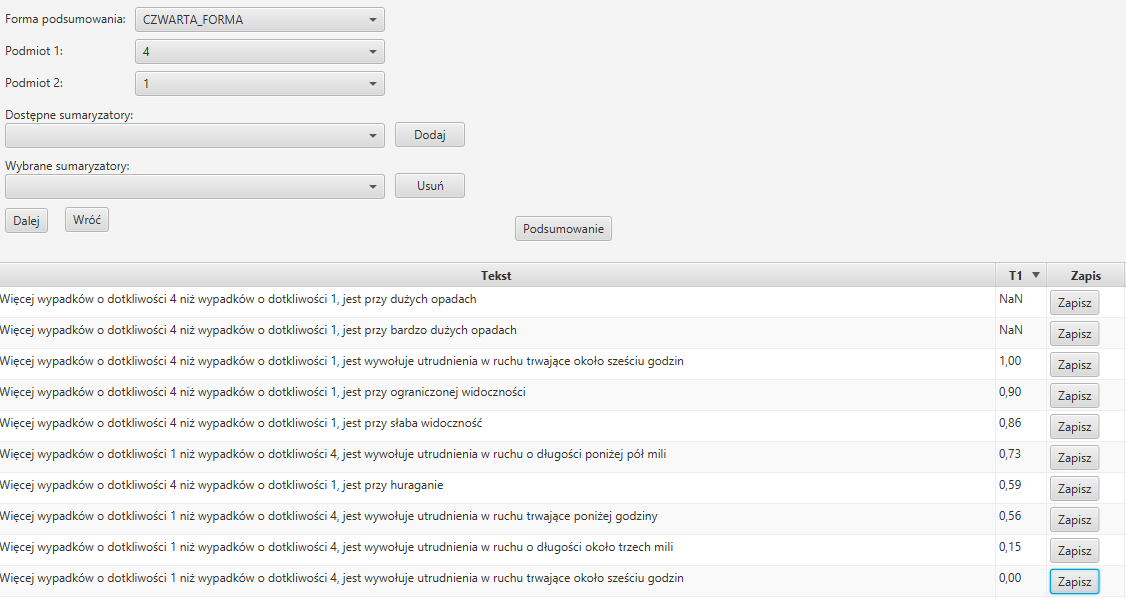
\includegraphics[width=15cm]{ex_wiel4.png}
 \vspace{-0.3cm}
 \caption{Tabela przedstawia wyniki wielopodmiotowych podsumowań lingwistycznych w czwartej formie dla eksperymentu 4. Kolumna Tekst zawiera tekst wygenerowanego wielopodmiotowego podsumowania lingwistycznego. Kolumna \textit{T\textsubscript{1}} zawiera wartość miary jakości \textit{T\textsubscript{1}} dla wielopodmiotowego podsumowania lignwistycznego \cite{niewiadomski19}. Ostatnia kolumna, Zapisz, zawiera przcisk zapisujący dane wielopodmiotowego podsumowania lignwistycznego do pliku. Każdy rząd zawiera jedno wygenerowane wielopodmiotowe podsumowanie lignwistyczne. Rzędy zostały posortowane po kolumnie \textit{T\textsubscript{1}} malejąco.  }
 \label{wykr_ex_wiel4}
\end{figure}


W czwartym eksperymencie wygenerowaliśmy wielopodmiotowe podsumowania lingwistyczne w czwartej formie. Wartość NaN w kolumnie \textit{T\textsubscript{1}} oznacza, że przynależność wypadków o zadanej dotkliwości do danego sumaryzatora wynosi 0 i następuje dzielenie przez 0. 

Na podstawie tabeli z Rysunku \ref{wykr_ex_wiel4} można zauważyć, że zdanie "Więcej wypadków o dotkliwości 4 niż wypadków o dotkliwości 1, jest wywołuje utrudnienia w ruchu trwające około sześciu godzin [1.00]" jest zdaniem najbardziej prawdziwym ze wszystkich wygenerowanych podsumowań w tym eksperymencie. Tak duża wartość miary \textit{T\textsubscript{1}} onacza, że zgodnie z naszymi przewidywaniami ilość wypadków o dotkliwości 1 wywołujących utrudnienia w ruchu trwające około sześciu godzin jest znikoma względem ilości wypadków o dotkliwości 4 wywołujących takie samo utrudnienie w ruchu drogowym. Zdanie, które uzyskało trzecią najwyższą wartość miary \textit{T\textsubscript{1}} jest zdanie: "Więcej wypadków o dotkliwości 4 niż wypadków o dotkliwości 1, jest przy słaba widoczność [0.86]". Wynik miary \textit{T\textsubscript{1}} dla wskazanego zdania jest zgodny z naszymi oczekiwaniami, ponieważ przy ograniczonej widoczności wystąpiło więcej wypadków o bardzo dużym wpływie na ruch drogowy, niż wypadków o małym wpływie na ruch drogowy. 


\newpage


%%%%%%%%%%%%%%%%%%%%%%%%%%%%%%%%%%%%%%%%%%%%%%%
\section{Dyskusja, wnioski}
\subsection{Dyskusja - Jednopodmiotowe podsumowania lingwistyczne}

\subsubsection{Jednopodmiotowe podsumowania lingwistyczne w pierwszej formie}

W sekcji \ref{section:ex} przeprowadziliśmy trzy eksperymenty. Sekcja \ref{section:ex1} była zapoznaniem z przeprowadzaniem podsumowań lingwistycznych. Zostały wygenerowane podsumowania lingwistyczne w pierwszej formie, badające związek ilości wypadków przy słabym wietrze oraz przy słąbym wietrze i umiarkowanych opadach. Przeprowadzone podsumowanie sprawdzające związek pomiędzy liczbą wypadków przy słabym wietrze, zgodnie z naszymi założeniami, około 1/3 wypadków miałoby miejsce przy słabym wietrze, co zostało potwierdzone przez podsumwoanie "Około 1/4 wypadków jest przy słabym wietrze [0.77]", dla którego miara \textit{T\textsubscript{1}} osiągneła wartość 0.92. Podczas przeprowadzania tego eksperymentu eksperymentowaliśmy z ustawieniem wag dla miar jakości podsumowań lingwistycznych, które ustawiliśmy na 0.65, 0.10, 0.04, 0.03, 0.03, 0.03, 0.03, 0.03, 0.03, 0.03, 0.00 odpowiednio dla miar od \textit{T\textsubscript{1}} do \textit{T\textsubscript{11}}. Waga dla miary \textit{T\textsubscript{11}} została ustawiona na 0.00, ponieważ wszystkie porównywane podsumowania lingwistyczne posiadają tą samą wartość 1.0. Natomaist miara \textit{T\textsubscript{1}} posiada największą wagę, ponieważ według nas jest najważniejszą miarą oceny jakości podsumowania. "Około 20 wypadków jest przy słabym wietrze, jest przy umiarkowanych opadach [0.68]" podsumowanie to osiągneło również wysoką wartość w prawdziwości zdania, oznacza to, że w naszym zbiorze danych występuje mało wypadków przy wcześniej wymienionych warunkach. \\

\subsubsection{Jednopodmiotowe podsumowania lingwistyczne w drugiej formie}

W sekcji \ref{section:ex2} wygenerowaliśmy jednopodmiotowe podsumowania lingwistyczne w drugiej formie - z klasyfikatorem. Przyjęliśmy takie wagi jakie zostały wymienione w dyskusji poprzedniego eksperymentu. W tym eksperymencie skupiliśmy sie na powiązaniu liczby wypadków z widocznością i ilością opadów. Zweryfikowaliśmy tezę, że wypadki będące przy dobrej widoczności są przy niewielkich opadach. Tą tezę udowodniło podsumowanie lingwistyczne: "Prawie wszystkie wypadków będących przy dobrej widoczności, jest przy niewielkich opadach [0.61]", dla którego miara \textit{T\textsubscript{1}} osiągnęła wartośc 0.69, a średnia ważona miar 0.61. Oznacza to, że tak jak założyliśmy, zdecydowana większość wypadków w naszym zbiorze danych, które były przy dobrej widoczności były przy dobrych opadach, czyli istnieje związek pomiędzy ilością opadów a widocznością. Następnie chcieliśmy zweryfikować tezę,  że wcześniej opiane warunki można powiązać z temperaturą oraz wilgotnością powietrza. Zgodnie z wynikiem podsumowania "Około połowy wypadków będących przy dobrej widoczności, jest przy niewielkich opadach, jest przy zimnej temperaturze [0.84]", które osiągneło bardzo wysokie wyniki miar jakości, dla miary \textit{T\textsubscript{1}} wynosiło 0.99, a dla średniej ważonej miar jakości 0.84. Wnioskujemy, że dobra widoczność oraz niskie opady idą w parze z niską temperaturą. Wbrew naszym oczekiwaniom nasza teza dotycząca zależności z wilgotnością powietrza nie potwierdziła się. Zgodnie z wynikami miar jakości podsumowania prawdą jest, żę : "Niewiele wypadków będących przy dobrej widoczności, jest przy niewielkich opadach, jest przy suchym powietrzu [0.18]". \\

W sekcji \ref{section:ex3} wygenerowaliśmy jednopodmiotowe podsumowania lingwistyczne w drugiej formie - z klasyfikatorem. Przyjęliśmy takie wagi jakie zostały wymienione w dyskusji poprzedniego eksperymentu. W tym eksperymencie skupiliśmy sie na powiązaniu długości ulicy posiadającej utrudnienia w ruchu drogowym spowodowanym przez wyapdek a czasem trwania utrudnień ruchu drogowego spowodowanymi przez wypadek. Przewidywaliśmy, że krótki odcinek drogi powoduje krótki czas utrudnień w ruchu drogowym. Teza została potwierdzona przez trzy podsumowania lingwistyczne: "Około połowy wypadków będących wywołuje utrudnienia w ruchu o długości poniżej pół mili, jest wywołuje utrudnienia w ruchu trwające około dwóch godzin [0.81]", "Niewiele wypadków będących wywołuje utrudnienia w ruchu o długości poniżej pół mili, jest wywołuje utrudnienia w ruchu trwające około sześciu godzin [0.81]", "Około 1/4 wypadków będących wywołuje utrudnienia w ruchu o długości poniżej pół mili, jest wywołuje utrudnienia w ruchu trwające poniżej godziny [0.62]" zgodnie z przewidywaniami podsumowania te uzyskały wysokie miary jakości podsumowania. Tak jak przewidywaliśmy w naszym zbiorze danych istnieje związek pomiędzy długością drogi dotkniętą utrudnieniami w ruchu drogowym a czasem trwania utrudnień w ruchu drogowym. 

\subsection{ Dyskusja - Wielopodmiotowe podsumowania lingwistyczne}

\subsubsection{Wielopodmiotowe podsumowania lingwistyczne w pierwszej formie}

W sekcji \ref{section:ex_wiel} przeprowadziliśmy cztery eksperymenty. W sekcji \ref{section:ex_wiel1} zostały wygenerowane wielopodmiotowe podsumowania lignwistyczne w pierwszej formie, badające związek ilości wypadków o dotkliwości 1 do wypadków o dotkliwości 4, które wywołały utrudnienia w ruchu o różnej długości. Zgodnie z naszymi oczekiwaniami najbardziej prawdziwym zdaniem, ze wszystkich wygenerowanych podsumowań, było zdanie: "Większość wypadków o dotkliwości 1 w odniesieniu do wypadków o dotkliwości 4, jest wywołuje utrudnienia w ruchu o długości poniżej pół mili [0,98]", oznacza to, że wypadki o mniejszym wpływie na utrudnienia ruchu drogowego powodowały mniejszą długość utrudnień w ruchu. Kolejnym wartym uwagi zdaniem było zdanie: "Około 1/4 wypadków o dotkliwości 1 w odniesieniu do wypadków o dotkliwości 4, jest wywołuje utrudnienia w ruchu o długości ponad trzech mili [0,65]", co obrazuje, że więcej wypadków o największym wpływie na utrudnienia w ruchu drogowym niż wypadków o najmniejszym wpływie na utrudnienia w ruchu drogowym powoduje utrudnienia w ruchu drogowym o najdłuższej długości, natomiast jest to mniejszy stosunek ilości wypadków niż w przypadku pierwszego zdania.\\

\subsubsection{Wielopodmiotowe podsumowania lingwistyczne w drugiej formie}

W sekcji \ref{section:ex_wiel2} zostały wygenerowane wielopodmiotowe podsumowania lignwistyczne w pierwszej oraz drugiej formie, badające związek ilości wypadków o dotkliwości 1 do wypadków o dotkliwości 2, które wywołały utrudnienia w ruchu trwające różną ilość godzin. Zdanie najbardziej prawdziwe z wygenerowanych podsumowań w pierwszej formie, to zdanie: "Większość wypadków o dotkliwości 1 w odniesieniu do wypadków o dotkliwości 2, jest wywołuje utrudnienia w ruchu trwające poniżej godziny [0,96]". Po dodaniu do opisanego zdania kwalifikatora  "wywołuje utrudnienia w ruchu o długości poniżej pół mili" zdanie staje się najmniej prawdziwe [0,00]. Dodanie kwalifikatora spowodowało ograniczenie drugiego podmiotu do wypadków, które mają największe prawdopodobieństwo spełnienia sumaryzatora. Wypadki, które posiadają dotkliwość 2 to najliczniejsza grupa wypadków, jest to grupa o najszerszej przynależności czasów trwania wypadków i długości na jaki mają wpływ i ograniczenie ich do wypadków, które spowodowały utrudnienia w ruchu poniżej pół mili spowodowało odfiltrowanie wielu wypadków powodujących długotrwałe utrudnienia w ruchu, co skutkuje znacznym zmniejszeniem jakości podsumowania. \\

\subsubsection{Wielopodmiotowe podsumowania lingwistyczne w trzeciej formie}

W sekcji \ref{section:ex_wiel3} zostały wygenerowane wielopodmiotowe podsumowania lignwistyczne w pierwszej oraz trzeciej formie. Zdanie "Większość wypadków o dotkliwości 1 w odniesieniu do wypadków o dotkliwości 2, jest przy niskim ciśnieniu [0,96]" posiada wysoką prawdziwość, natomiast po dodaniu do zdania kwalifikatora "będących przy bardzo ciepłej temperaturze" powoduje znaczny spadek prawdziwości zdania, wynika z tego, że jeśli wypadki były przy niskim ciśnieniu to temperatura powietrza w trakcie wypadku nie była ciepła. W przypadku zdania "Większość wypadków o dotkliwości 2 w odniesieniu do wypadków o dotkliwości 3, jest wywołuje utrudnienia w ruchu trwające około czterech godzin [0,01]" dodanie kwalifikatora "będących wywołuje utrudnienia w ruchu o długości około jednej mili" spowodowało znaczne zmniejszenie prawdziwości zdania. \\

\subsubsection{Wielopodmiotowe podsumowania lingwistyczne w czwartej formie}

W sekcji \ref{section:ex_wiel4} zostały wygenerowane wielopodmiotowe podsumowania lignwistyczne w czwartej formie porównujące wypadki o dotkliwości 1 z wypadkami o dotkliwości 4, czyli wypadki znajdujące się na dwóch ekstremach skali dotlkiwości. Chcieliśmy potweirdzić naszą tezę, że wypadki o dotkliwości 4 występowały przy bardziej ekstremalnych warunkach atmosferycznych, a także, że miały większy wpływ na ruch drogowy. Według nas najważniejsze z wygenerowanych podsumowań to: "Więcej wypadków o dotkliwości 4 niż wypadków o dotkliwości 1, jest wywołuje utrudnienia w ruchu trwające około sześciu godzin [1,00]", "Więcej wypadków o dotkliwości 4 niż wypadków o dotkliwości 1, jest przy ograniczonej widoczności [0,90]", "Więcej wypadków o dotkliwości 4 niż wypadków o dotkliwości 1, jest przy słaba widoczność [0,86]", "Więcej wypadków o dotkliwości 1 niż wypadków o dotkliwości 4, jest wywołuje utrudnienia w ruchu o długości poniżej pół mili [0,73]". Zgodnie z naszymi przewidywaniami wygenerowane podsumowania uzyskały wysoki poziom prawdziwości. Potwierdza to wcześniej przedstawione przez nas przewidywania odnosie analizowanego zbioru danych.  


\subsection{Wnioski}

\begin{itemize}
\item Najważniejszą miarą jakości dla podsumowań lingwistycznych jest miara \textit{T\textsubscript{1}} -  stopień prawdziwości.
\item Odpowiednio dobrane do badanego zbioru danych podsumowanie lingwistyczne pozwala na uzsykanie wielu cennych informacji dot. dango zbioru.
\item Dla każdego badanego zbioru danych należy indywidualnie dobrać kwantyfikatory absolutne oraz klasyfikatory/sumaryzatory.
\item Dobór kwantyfikatorów absolutnych zależy od ilości badanych elementów w zbiorze danych.
\item Jednopodmiotowe podsumowania lingwistyczne w pierwszej formie dostarcza bardziej ogólnych danych niż w drugiej formie, ale jest łatwiejsze do skonstruowania i zrozumienia.
\item Wielopodmiotowe podsumowania lingwistyczne pozwalają nam na łatwe podzielenie zbioru danych według wybranej cechy i porównanie tak podzielonych zbiorów.
\item Im węższe przedziały przynależności funkcji przynależności tym dokładniejsze informacje uzyskujemy z podsumowań.
\item Słaba widoczność idzie w parze z dużymi opadami deszczu.
\item Im dłuższy czas trwania utrudnień na drodze wywołanych przez wypadek tym średnio dłuższy odcinek drogi dotknięty wypadkiem.
\item Wypadki o większej dotkliwości zazwyczaj są przy gorszych warunkach niż te o mniejszej dotkliwości
\end{itemize}



%%%%%%%%%%%%%%%%%%%%%%%%%%%%%%%%%%%%%%%%%%%%%%%
\section{Braki w realizacji projektu 2.}
Wszystkie obowiązkowe elementy projektu zostały zrealizowane.



\begin{thebibliography}{99}
\bibitem{przyklad} I. Superson, A. Niewiadomski, POZYSKIWANIE WIEDZY Z RELACYJNYCH BAZ DANYCH: WIELOPODMIOTOWE PODSUMOWANIA LINGWISTYCZNE, Politechnika Łódzka
\bibitem{niewiadomskiRozmyte} A. Niewiadomski, Rozmyte metody inteligentnej interpretacji danych, tom 10, 2006, 546-547
\bibitem{dane} 2021 Kaggle Inc [internetowa społeczność związana z analizą danych], US Accidents (3 million records -- updated)
A Countrywide Traffic Accident Dataset (2016 - 2020) [przeglądany 24 kwietnia 2021], Dostępny w: \url{https://www.kaggle.com/sobhanmoosavi/us-accidents}
Oficyna Wydawnicza EXIT, Warszawa, 2008.
\bibitem{fuzzy} Zadeh L.A., A computational approach to fuzzy quantifiers in natural languages. Computers and Maths with Applications, nr 9, 1983, 149-183
 \bibitem{niewiadomski19} A. Niewiadomski, Zbiory rozmyte typu 2. Zastosowania w reprezentowaniu informacji.  Seria „Problemy współczesnej informatyki” pod redakcją L. Rutkowskiego. Akademicka Oficyna Wydawnicza EXIT, Warszawa, 2019.
\bibitem{zadrozny06} S. Zadrożny, Zapytania nieprecyzyjne i lingwistyczne podsumowania baz danych, EXIT, 2006, Warszawa
\bibitem{niewiadomski08} A. Niewiadomski, Methods for the Linguistic Summarization of Data: Applications of Fuzzy Sets and Their Extensions, Akademicka 
\bibitem{fuzzySet} Zadeh, L. A.: 1965, ‘Fuzzy sets’. Inf. and Control 8, 338–353.
\bibitem{broniarska} dr inż. Anna Bryniarska, Podstawy teorii systemów rozmytych z zadaniami, Dostępny w: \url{https://a.bryniarska.po.opole.pl/images/nsi/skrypt_r2_28listopada.pdf},
\bibitem{niewiadomski zbiory rozmyte typu 2}{ Niewiadomski, Adam. Zbiory rozmyte typu 2. Zastosowania w reprezentacji informacji. Red. . : Akademicka Oficyna Wydawnicza EXIT Andrzej Lang, 2019, 195 s. ISBN 978-83-7837-595-1 } 
\end{thebibliography}

Literatura zawiera wyłącznie źródła recenzowane i/lub o potwierdzonej wiarygodności,
możliwe do weryfikacji i cytowane w sprawozdaniu. 
\end{document}
